
% Default to the notebook output style

    


% Inherit from the specified cell style.




    
\documentclass[11pt]{article}
\input glyphtounicode\pdfgentounicode=1
\usepackage{dhucs}
\SetHangulFonts{utbt}{utgt}{utgt}
    
    
    \usepackage[T1]{fontenc}
    % Nicer default font than Computer Modern for most use cases
    \usepackage{palatino}

    % Basic figure setup, for now with no caption control since it's done
    % automatically by Pandoc (which extracts ![](path) syntax from Markdown).
    \usepackage{graphicx}
    % We will generate all images so they have a width \maxwidth. This means
    % that they will get their normal width if they fit onto the page, but
    % are scaled down if they would overflow the margins.
    \makeatletter
    \def\maxwidth{\ifdim\Gin@nat@width>\linewidth\linewidth
    \else\Gin@nat@width\fi}
    \makeatother
    \let\Oldincludegraphics\includegraphics
    % Set max figure width to be 80% of text width, for now hardcoded.
    \renewcommand{\includegraphics}[1]{\Oldincludegraphics[width=.8\maxwidth]{#1}}
    % Ensure that by default, figures have no caption (until we provide a
    % proper Figure object with a Caption API and a way to capture that
    % in the conversion process - todo).
    \usepackage{caption}
    \DeclareCaptionLabelFormat{nolabel}{}
    \captionsetup{labelformat=nolabel}

    \usepackage{adjustbox} % Used to constrain images to a maximum size 
    \usepackage{xcolor} % Allow colors to be defined
    \usepackage{enumerate} % Needed for markdown enumerations to work
    \usepackage{geometry} % Used to adjust the document margins
    \usepackage{amsmath} % Equations
    \usepackage{amssymb} % Equations
    \usepackage{textcomp} % defines textquotesingle
    % Hack from http://tex.stackexchange.com/a/47451/13684:
    \AtBeginDocument{%
        \def\PYZsq{\textquotesingle}% Upright quotes in Pygmentized code
    }
    \usepackage{upquote} % Upright quotes for verbatim code
    \usepackage{eurosym} % defines \euro
    \usepackage[mathletters]{ucs} % Extended unicode (utf-8) support
    \usepackage[utf8x]{inputenc} % Allow utf-8 characters in the tex document
    \usepackage{fancyvrb} % verbatim replacement that allows latex
    \usepackage{grffile} % extends the file name processing of package graphics 
                         % to support a larger range 
    % The hyperref package gives us a pdf with properly built
    % internal navigation ('pdf bookmarks' for the table of contents,
    % internal cross-reference links, web links for URLs, etc.)
    \usepackage{hyperref}
    \usepackage{longtable} % longtable support required by pandoc >1.10
    \usepackage{booktabs}  % table support for pandoc > 1.12.2
    \usepackage[normalem]{ulem} % ulem is needed to support strikethroughs (\sout)
                                % normalem makes italics be italics, not underlines
    

    
    
    % Colors for the hyperref package
    \definecolor{urlcolor}{rgb}{0,.145,.698}
    \definecolor{linkcolor}{rgb}{.71,0.21,0.01}
    \definecolor{citecolor}{rgb}{.12,.54,.11}

    % ANSI colors
    \definecolor{ansi-black}{HTML}{3E424D}
    \definecolor{ansi-black-intense}{HTML}{282C36}
    \definecolor{ansi-red}{HTML}{E75C58}
    \definecolor{ansi-red-intense}{HTML}{B22B31}
    \definecolor{ansi-green}{HTML}{00A250}
    \definecolor{ansi-green-intense}{HTML}{007427}
    \definecolor{ansi-yellow}{HTML}{DDB62B}
    \definecolor{ansi-yellow-intense}{HTML}{B27D12}
    \definecolor{ansi-blue}{HTML}{208FFB}
    \definecolor{ansi-blue-intense}{HTML}{0065CA}
    \definecolor{ansi-magenta}{HTML}{D160C4}
    \definecolor{ansi-magenta-intense}{HTML}{A03196}
    \definecolor{ansi-cyan}{HTML}{60C6C8}
    \definecolor{ansi-cyan-intense}{HTML}{258F8F}
    \definecolor{ansi-white}{HTML}{C5C1B4}
    \definecolor{ansi-white-intense}{HTML}{A1A6B2}

    % commands and environments needed by pandoc snippets
    % extracted from the output of `pandoc -s`
    \providecommand{\tightlist}{%
      \setlength{\itemsep}{0pt}\setlength{\parskip}{0pt}}
    \DefineVerbatimEnvironment{Highlighting}{Verbatim}{commandchars=\\\{\}}
    % Add ',fontsize=\small' for more characters per line
    \newenvironment{Shaded}{}{}
    \newcommand{\KeywordTok}[1]{\textcolor[rgb]{0.00,0.44,0.13}{\textbf{{#1}}}}
    \newcommand{\DataTypeTok}[1]{\textcolor[rgb]{0.56,0.13,0.00}{{#1}}}
    \newcommand{\DecValTok}[1]{\textcolor[rgb]{0.25,0.63,0.44}{{#1}}}
    \newcommand{\BaseNTok}[1]{\textcolor[rgb]{0.25,0.63,0.44}{{#1}}}
    \newcommand{\FloatTok}[1]{\textcolor[rgb]{0.25,0.63,0.44}{{#1}}}
    \newcommand{\CharTok}[1]{\textcolor[rgb]{0.25,0.44,0.63}{{#1}}}
    \newcommand{\StringTok}[1]{\textcolor[rgb]{0.25,0.44,0.63}{{#1}}}
    \newcommand{\CommentTok}[1]{\textcolor[rgb]{0.38,0.63,0.69}{\textit{{#1}}}}
    \newcommand{\OtherTok}[1]{\textcolor[rgb]{0.00,0.44,0.13}{{#1}}}
    \newcommand{\AlertTok}[1]{\textcolor[rgb]{1.00,0.00,0.00}{\textbf{{#1}}}}
    \newcommand{\FunctionTok}[1]{\textcolor[rgb]{0.02,0.16,0.49}{{#1}}}
    \newcommand{\RegionMarkerTok}[1]{{#1}}
    \newcommand{\ErrorTok}[1]{\textcolor[rgb]{1.00,0.00,0.00}{\textbf{{#1}}}}
    \newcommand{\NormalTok}[1]{{#1}}
    
    % Additional commands for more recent versions of Pandoc
    \newcommand{\ConstantTok}[1]{\textcolor[rgb]{0.53,0.00,0.00}{{#1}}}
    \newcommand{\SpecialCharTok}[1]{\textcolor[rgb]{0.25,0.44,0.63}{{#1}}}
    \newcommand{\VerbatimStringTok}[1]{\textcolor[rgb]{0.25,0.44,0.63}{{#1}}}
    \newcommand{\SpecialStringTok}[1]{\textcolor[rgb]{0.73,0.40,0.53}{{#1}}}
    \newcommand{\ImportTok}[1]{{#1}}
    \newcommand{\DocumentationTok}[1]{\textcolor[rgb]{0.73,0.13,0.13}{\textit{{#1}}}}
    \newcommand{\AnnotationTok}[1]{\textcolor[rgb]{0.38,0.63,0.69}{\textbf{\textit{{#1}}}}}
    \newcommand{\CommentVarTok}[1]{\textcolor[rgb]{0.38,0.63,0.69}{\textbf{\textit{{#1}}}}}
    \newcommand{\VariableTok}[1]{\textcolor[rgb]{0.10,0.09,0.49}{{#1}}}
    \newcommand{\ControlFlowTok}[1]{\textcolor[rgb]{0.00,0.44,0.13}{\textbf{{#1}}}}
    \newcommand{\OperatorTok}[1]{\textcolor[rgb]{0.40,0.40,0.40}{{#1}}}
    \newcommand{\BuiltInTok}[1]{{#1}}
    \newcommand{\ExtensionTok}[1]{{#1}}
    \newcommand{\PreprocessorTok}[1]{\textcolor[rgb]{0.74,0.48,0.00}{{#1}}}
    \newcommand{\AttributeTok}[1]{\textcolor[rgb]{0.49,0.56,0.16}{{#1}}}
    \newcommand{\InformationTok}[1]{\textcolor[rgb]{0.38,0.63,0.69}{\textbf{\textit{{#1}}}}}
    \newcommand{\WarningTok}[1]{\textcolor[rgb]{0.38,0.63,0.69}{\textbf{\textit{{#1}}}}}
    
    
    % Define a nice break command that doesn't care if a line doesn't already
    % exist.
    \def\br{\hspace*{\fill} \\* }
    % Math Jax compatability definitions
    \def\gt{>}
    \def\lt{<}
    % Document parameters
    \title{Learning Spark\_Chapter6}
    
    
    

    % Pygments definitions
    
\makeatletter
\def\PY@reset{\let\PY@it=\relax \let\PY@bf=\relax%
    \let\PY@ul=\relax \let\PY@tc=\relax%
    \let\PY@bc=\relax \let\PY@ff=\relax}
\def\PY@tok#1{\csname PY@tok@#1\endcsname}
\def\PY@toks#1+{\ifx\relax#1\empty\else%
    \PY@tok{#1}\expandafter\PY@toks\fi}
\def\PY@do#1{\PY@bc{\PY@tc{\PY@ul{%
    \PY@it{\PY@bf{\PY@ff{#1}}}}}}}
\def\PY#1#2{\PY@reset\PY@toks#1+\relax+\PY@do{#2}}

\expandafter\def\csname PY@tok@gd\endcsname{\def\PY@tc##1{\textcolor[rgb]{0.63,0.00,0.00}{##1}}}
\expandafter\def\csname PY@tok@gu\endcsname{\let\PY@bf=\textbf\def\PY@tc##1{\textcolor[rgb]{0.50,0.00,0.50}{##1}}}
\expandafter\def\csname PY@tok@gt\endcsname{\def\PY@tc##1{\textcolor[rgb]{0.00,0.27,0.87}{##1}}}
\expandafter\def\csname PY@tok@gs\endcsname{\let\PY@bf=\textbf}
\expandafter\def\csname PY@tok@gr\endcsname{\def\PY@tc##1{\textcolor[rgb]{1.00,0.00,0.00}{##1}}}
\expandafter\def\csname PY@tok@cm\endcsname{\let\PY@it=\textit\def\PY@tc##1{\textcolor[rgb]{0.25,0.50,0.50}{##1}}}
\expandafter\def\csname PY@tok@vg\endcsname{\def\PY@tc##1{\textcolor[rgb]{0.10,0.09,0.49}{##1}}}
\expandafter\def\csname PY@tok@vi\endcsname{\def\PY@tc##1{\textcolor[rgb]{0.10,0.09,0.49}{##1}}}
\expandafter\def\csname PY@tok@mh\endcsname{\def\PY@tc##1{\textcolor[rgb]{0.40,0.40,0.40}{##1}}}
\expandafter\def\csname PY@tok@cs\endcsname{\let\PY@it=\textit\def\PY@tc##1{\textcolor[rgb]{0.25,0.50,0.50}{##1}}}
\expandafter\def\csname PY@tok@ge\endcsname{\let\PY@it=\textit}
\expandafter\def\csname PY@tok@vc\endcsname{\def\PY@tc##1{\textcolor[rgb]{0.10,0.09,0.49}{##1}}}
\expandafter\def\csname PY@tok@il\endcsname{\def\PY@tc##1{\textcolor[rgb]{0.40,0.40,0.40}{##1}}}
\expandafter\def\csname PY@tok@go\endcsname{\def\PY@tc##1{\textcolor[rgb]{0.53,0.53,0.53}{##1}}}
\expandafter\def\csname PY@tok@cp\endcsname{\def\PY@tc##1{\textcolor[rgb]{0.74,0.48,0.00}{##1}}}
\expandafter\def\csname PY@tok@gi\endcsname{\def\PY@tc##1{\textcolor[rgb]{0.00,0.63,0.00}{##1}}}
\expandafter\def\csname PY@tok@gh\endcsname{\let\PY@bf=\textbf\def\PY@tc##1{\textcolor[rgb]{0.00,0.00,0.50}{##1}}}
\expandafter\def\csname PY@tok@ni\endcsname{\let\PY@bf=\textbf\def\PY@tc##1{\textcolor[rgb]{0.60,0.60,0.60}{##1}}}
\expandafter\def\csname PY@tok@nl\endcsname{\def\PY@tc##1{\textcolor[rgb]{0.63,0.63,0.00}{##1}}}
\expandafter\def\csname PY@tok@nn\endcsname{\let\PY@bf=\textbf\def\PY@tc##1{\textcolor[rgb]{0.00,0.00,1.00}{##1}}}
\expandafter\def\csname PY@tok@no\endcsname{\def\PY@tc##1{\textcolor[rgb]{0.53,0.00,0.00}{##1}}}
\expandafter\def\csname PY@tok@na\endcsname{\def\PY@tc##1{\textcolor[rgb]{0.49,0.56,0.16}{##1}}}
\expandafter\def\csname PY@tok@nb\endcsname{\def\PY@tc##1{\textcolor[rgb]{0.00,0.50,0.00}{##1}}}
\expandafter\def\csname PY@tok@nc\endcsname{\let\PY@bf=\textbf\def\PY@tc##1{\textcolor[rgb]{0.00,0.00,1.00}{##1}}}
\expandafter\def\csname PY@tok@nd\endcsname{\def\PY@tc##1{\textcolor[rgb]{0.67,0.13,1.00}{##1}}}
\expandafter\def\csname PY@tok@ne\endcsname{\let\PY@bf=\textbf\def\PY@tc##1{\textcolor[rgb]{0.82,0.25,0.23}{##1}}}
\expandafter\def\csname PY@tok@nf\endcsname{\def\PY@tc##1{\textcolor[rgb]{0.00,0.00,1.00}{##1}}}
\expandafter\def\csname PY@tok@si\endcsname{\let\PY@bf=\textbf\def\PY@tc##1{\textcolor[rgb]{0.73,0.40,0.53}{##1}}}
\expandafter\def\csname PY@tok@s2\endcsname{\def\PY@tc##1{\textcolor[rgb]{0.73,0.13,0.13}{##1}}}
\expandafter\def\csname PY@tok@nt\endcsname{\let\PY@bf=\textbf\def\PY@tc##1{\textcolor[rgb]{0.00,0.50,0.00}{##1}}}
\expandafter\def\csname PY@tok@nv\endcsname{\def\PY@tc##1{\textcolor[rgb]{0.10,0.09,0.49}{##1}}}
\expandafter\def\csname PY@tok@s1\endcsname{\def\PY@tc##1{\textcolor[rgb]{0.73,0.13,0.13}{##1}}}
\expandafter\def\csname PY@tok@ch\endcsname{\let\PY@it=\textit\def\PY@tc##1{\textcolor[rgb]{0.25,0.50,0.50}{##1}}}
\expandafter\def\csname PY@tok@m\endcsname{\def\PY@tc##1{\textcolor[rgb]{0.40,0.40,0.40}{##1}}}
\expandafter\def\csname PY@tok@gp\endcsname{\let\PY@bf=\textbf\def\PY@tc##1{\textcolor[rgb]{0.00,0.00,0.50}{##1}}}
\expandafter\def\csname PY@tok@sh\endcsname{\def\PY@tc##1{\textcolor[rgb]{0.73,0.13,0.13}{##1}}}
\expandafter\def\csname PY@tok@ow\endcsname{\let\PY@bf=\textbf\def\PY@tc##1{\textcolor[rgb]{0.67,0.13,1.00}{##1}}}
\expandafter\def\csname PY@tok@sx\endcsname{\def\PY@tc##1{\textcolor[rgb]{0.00,0.50,0.00}{##1}}}
\expandafter\def\csname PY@tok@bp\endcsname{\def\PY@tc##1{\textcolor[rgb]{0.00,0.50,0.00}{##1}}}
\expandafter\def\csname PY@tok@c1\endcsname{\let\PY@it=\textit\def\PY@tc##1{\textcolor[rgb]{0.25,0.50,0.50}{##1}}}
\expandafter\def\csname PY@tok@o\endcsname{\def\PY@tc##1{\textcolor[rgb]{0.40,0.40,0.40}{##1}}}
\expandafter\def\csname PY@tok@kc\endcsname{\let\PY@bf=\textbf\def\PY@tc##1{\textcolor[rgb]{0.00,0.50,0.00}{##1}}}
\expandafter\def\csname PY@tok@c\endcsname{\let\PY@it=\textit\def\PY@tc##1{\textcolor[rgb]{0.25,0.50,0.50}{##1}}}
\expandafter\def\csname PY@tok@mf\endcsname{\def\PY@tc##1{\textcolor[rgb]{0.40,0.40,0.40}{##1}}}
\expandafter\def\csname PY@tok@err\endcsname{\def\PY@bc##1{\setlength{\fboxsep}{0pt}\fcolorbox[rgb]{1.00,0.00,0.00}{1,1,1}{\strut ##1}}}
\expandafter\def\csname PY@tok@mb\endcsname{\def\PY@tc##1{\textcolor[rgb]{0.40,0.40,0.40}{##1}}}
\expandafter\def\csname PY@tok@ss\endcsname{\def\PY@tc##1{\textcolor[rgb]{0.10,0.09,0.49}{##1}}}
\expandafter\def\csname PY@tok@sr\endcsname{\def\PY@tc##1{\textcolor[rgb]{0.73,0.40,0.53}{##1}}}
\expandafter\def\csname PY@tok@mo\endcsname{\def\PY@tc##1{\textcolor[rgb]{0.40,0.40,0.40}{##1}}}
\expandafter\def\csname PY@tok@kd\endcsname{\let\PY@bf=\textbf\def\PY@tc##1{\textcolor[rgb]{0.00,0.50,0.00}{##1}}}
\expandafter\def\csname PY@tok@mi\endcsname{\def\PY@tc##1{\textcolor[rgb]{0.40,0.40,0.40}{##1}}}
\expandafter\def\csname PY@tok@kn\endcsname{\let\PY@bf=\textbf\def\PY@tc##1{\textcolor[rgb]{0.00,0.50,0.00}{##1}}}
\expandafter\def\csname PY@tok@cpf\endcsname{\let\PY@it=\textit\def\PY@tc##1{\textcolor[rgb]{0.25,0.50,0.50}{##1}}}
\expandafter\def\csname PY@tok@kr\endcsname{\let\PY@bf=\textbf\def\PY@tc##1{\textcolor[rgb]{0.00,0.50,0.00}{##1}}}
\expandafter\def\csname PY@tok@s\endcsname{\def\PY@tc##1{\textcolor[rgb]{0.73,0.13,0.13}{##1}}}
\expandafter\def\csname PY@tok@kp\endcsname{\def\PY@tc##1{\textcolor[rgb]{0.00,0.50,0.00}{##1}}}
\expandafter\def\csname PY@tok@w\endcsname{\def\PY@tc##1{\textcolor[rgb]{0.73,0.73,0.73}{##1}}}
\expandafter\def\csname PY@tok@kt\endcsname{\def\PY@tc##1{\textcolor[rgb]{0.69,0.00,0.25}{##1}}}
\expandafter\def\csname PY@tok@sc\endcsname{\def\PY@tc##1{\textcolor[rgb]{0.73,0.13,0.13}{##1}}}
\expandafter\def\csname PY@tok@sb\endcsname{\def\PY@tc##1{\textcolor[rgb]{0.73,0.13,0.13}{##1}}}
\expandafter\def\csname PY@tok@k\endcsname{\let\PY@bf=\textbf\def\PY@tc##1{\textcolor[rgb]{0.00,0.50,0.00}{##1}}}
\expandafter\def\csname PY@tok@se\endcsname{\let\PY@bf=\textbf\def\PY@tc##1{\textcolor[rgb]{0.73,0.40,0.13}{##1}}}
\expandafter\def\csname PY@tok@sd\endcsname{\let\PY@it=\textit\def\PY@tc##1{\textcolor[rgb]{0.73,0.13,0.13}{##1}}}

\def\PYZbs{\char`\\}
\def\PYZus{\char`\_}
\def\PYZob{\char`\{}
\def\PYZcb{\char`\}}
\def\PYZca{\char`\^}
\def\PYZam{\char`\&}
\def\PYZlt{\char`\<}
\def\PYZgt{\char`\>}
\def\PYZsh{\char`\#}
\def\PYZpc{\char`\%}
\def\PYZdl{\char`\$}
\def\PYZhy{\char`\-}
\def\PYZsq{\char`\'}
\def\PYZdq{\char`\"}
\def\PYZti{\char`\~}
% for compatibility with earlier versions
\def\PYZat{@}
\def\PYZlb{[}
\def\PYZrb{]}
\makeatother


    % Exact colors from NB
    \definecolor{incolor}{rgb}{0.0, 0.0, 0.5}
    \definecolor{outcolor}{rgb}{0.545, 0.0, 0.0}



    
    % Prevent overflowing lines due to hard-to-break entities
    \sloppy 
    % Setup hyperref package
    \hypersetup{
      breaklinks=true,  % so long urls are correctly broken across lines
      colorlinks=true,
      urlcolor=urlcolor,
      linkcolor=linkcolor,
      citecolor=citecolor,
      }
    % Slightly bigger margins than the latex defaults
    
    \geometry{verbose,tmargin=1in,bmargin=1in,lmargin=1in,rmargin=1in}
    
    

    \begin{document}
    
    
    \maketitle
    
    

    
    \section{Chapter 6. Advanced Spark
Progamming}\label{chapter-6.-advanced-spark-progamming}

    \subsubsection{소개}\label{uxc18cuxac1c}

    이 장에서는 아래 4가지를 배우게 됨 \textgreater{} - Accumulator
\textgreater{} - Broadcast variable \textgreater{} - 파티션 단위
Transformation (mapPartitions, mapPartitionsWithIndex,
foreachPartition() \textgreater{} - pipe()을 이용한 외부 스크립트 활용

    \begin{quote}
샘플 데이터로는 아래와 같은 ham radio call log를 사용.. 하려 했으나 원본
파일을 구할수 없음..\\대신 Spark 설치시 만들어지는 README.md 파일 사용
\end{quote}

    \begin{Verbatim}[commandchars=\\\{\}]
{\color{incolor}In [{\color{incolor}1}]:} \PY{k}{import} \PY{n+nn}{play.api.libs.json.\PYZus{}}
        
        \PY{k}{val} \PY{n}{call} \PY{k}{=} \PY{l+s}{\PYZdq{}\PYZdq{}\PYZdq{}\PYZob{}\PYZdq{}address\PYZdq{}:\PYZdq{}address here\PYZdq{}, \PYZdq{}band\PYZdq{}:\PYZdq{}40m\PYZdq{},\PYZdq{}callsign\PYZdq{}:\PYZdq{}KK6JLK\PYZdq{},\PYZdq{}city\PYZdq{}:\PYZdq{}SUNNYVALE\PYZdq{},}
        \PY{l+s}{\PYZdq{}contactlat\PYZdq{}:\PYZdq{}37.384733\PYZdq{},\PYZdq{}contactlong\PYZdq{}:\PYZdq{}\PYZhy{}122.032164\PYZdq{},}
        \PY{l+s}{\PYZdq{}county\PYZdq{}:\PYZdq{}Santa Clara\PYZdq{},\PYZdq{}dxcc\PYZdq{}:\PYZdq{}291\PYZdq{},\PYZdq{}fullname\PYZdq{}:\PYZdq{}MATTHEW McPherrin\PYZdq{},}
        \PY{l+s}{\PYZdq{}id\PYZdq{}:57779,\PYZdq{}mode\PYZdq{}:\PYZdq{}FM\PYZdq{},\PYZdq{}mylat\PYZdq{}:\PYZdq{}37.751952821\PYZdq{},\PYZdq{}mylong\PYZdq{}:\PYZdq{}\PYZhy{}122.4208688735\PYZdq{}\PYZcb{}\PYZdq{}\PYZdq{}\PYZdq{}}
        
        \PY{n}{print}\PY{o}{(}\PY{n}{call}\PY{o}{)}
\end{Verbatim}

    \begin{Verbatim}[commandchars=\\\{\}]
\{"address":"address here", "band":"40m","callsign":"KK6JLK","city":"SUNNYVALE",
"contactlat":"37.384733","contactlong":"-122.032164",
"county":"Santa Clara","dxcc":"291","fullname":"MATTHEW McPherrin",
"id":57779,"mode":"FM","mylat":"37.751952821","mylong":"-122.4208688735"\}
    \end{Verbatim}

    \subsubsection{어큐뮬레이터(Accumulators)}\label{uxc5b4uxd050uxbbacuxb808uxc774uxd130accumulators}

    \begin{quote}
Spark에서 제공하는 shared variable에는 \textbf{accumulator}와
\textbf{broadcast variable}가 있다.
\end{quote}

\begin{quote}
\textbf{accumulator}는 그 이름이 의미하는 것 처럼\\Cluster에 분산되어
있는 각 worker node에서 일어나는\\어떤 이벤트의 수를 카운트하여 driver
program에 집계하는 것과 같은 목적으로 사용한다.
\end{quote}

\begin{quote}
물론 RDD Transformation으로도 각 worker node에서 driver program으로
동일한 정보 집계를 구현할 수 있으나\\원래 목적으로 하는 RDD
Transformation에 비해\\다소 보조적인 목적(디버깅, 모니터링)을 위해
사용하며\\마치 전체 cluster 전역변수를 사용하는 것과 같이 간단한
문법으로 사용할 수 있다.
\end{quote}

    \begin{figure}[htbp]
\centering
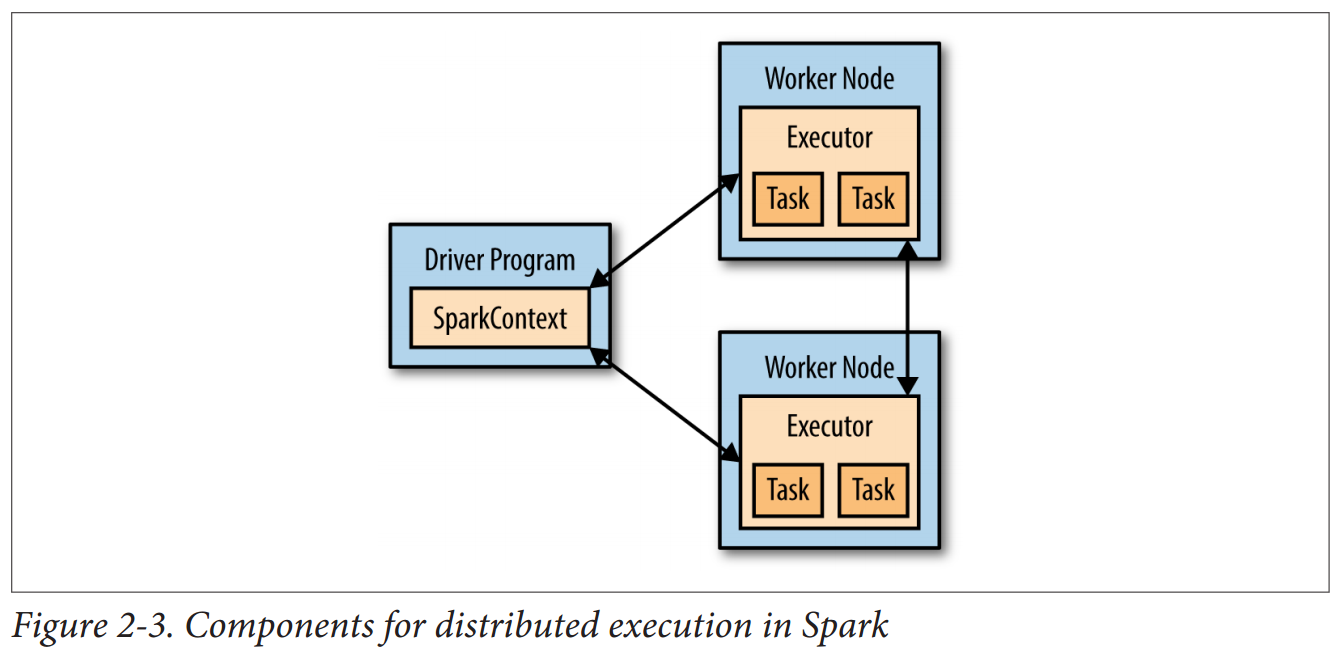
\includegraphics{./_images/figure_2_3.PNG}
\caption{Local image}
\end{figure}

    Example: simple accumulator

    \begin{quote}
\textbf{accumulator} 생성은 아래와 같으며, accumulator에 초기값을
할당하고, 초기값의 Type에 따른 그 동작이 다르다.\\(아래 예 에서는
org.apache.spark.Accumulator$<java.lang.Integer>$ type의 object가
생성된다.)
\end{quote}

\begin{Shaded}
\begin{Highlighting}[]
\KeywordTok{val} \NormalTok{blankLines = sc.}\FunctionTok{accumulator}\NormalTok{(}\DecValTok{0}\NormalTok{)}
\end{Highlighting}
\end{Shaded}

\begin{quote}
Worker node에서 \textbf{accumulator}변수에 += 연산을 이용하여 값을 더할
수 있다.
\end{quote}

    \begin{Verbatim}[commandchars=\\\{\}]
{\color{incolor}In [{\color{incolor}2}]:} \PY{k}{val} \PY{n}{file} \PY{k}{=} \PY{n}{sc}\PY{o}{.}\PY{n}{textFile}\PY{o}{(}\PY{l+s}{\PYZdq{}/home/sparkuser/spark\PYZhy{}1.6.2\PYZhy{}bin\PYZhy{}hadoop2.6/README.md\PYZdq{}}\PY{o}{)}
        \PY{n}{file}\PY{o}{.}
          \PY{n}{take}\PY{o}{(}\PY{l+m+mi}{10}\PY{o}{)}\PY{o}{.}
          \PY{n}{foreach}\PY{o}{(}\PY{n}{println}\PY{o}{)}
          
        \PY{n}{print}\PY{o}{(}\PY{l+s}{\PYZdq{}\PYZbs{}nNumber of partitions: \PYZdq{}} \PY{o}{+} \PY{n}{file}\PY{o}{.}\PY{n}{partitions}\PY{o}{.}\PY{n}{size}\PY{o}{)}
\end{Verbatim}

    \begin{Verbatim}[commandchars=\\\{\}]
\# Apache Spark

Spark is a fast and general cluster computing system for Big Data. It provides
high-level APIs in Scala, Java, Python, and R, and an optimized engine that
supports general computation graphs for data analysis. It also supports a
rich set of higher-level tools including Spark SQL for SQL and DataFrames,
MLlib for machine learning, GraphX for graph processing,
and Spark Streaming for stream processing.

<http://spark.apache.org/>

Number of partitions: 1
    \end{Verbatim}

    \begin{Verbatim}[commandchars=\\\{\}]
{\color{incolor}In [{\color{incolor}26}]:} \PY{k}{val} \PY{n}{blankLines} \PY{k}{=} \PY{n}{sc}\PY{o}{.}\PY{n}{accumulator}\PY{o}{(}\PY{l+m+mi}{0}\PY{o}{,} \PY{l+s}{\PYZdq{}counter\PYZdq{}}\PY{o}{)}
         
         \PY{k}{val} \PY{n}{callSigns} \PY{k}{=} \PY{n}{file}\PY{o}{.}\PY{n}{flatMap}\PY{o}{(}\PY{n}{line} \PY{k}{=\PYZgt{}} \PY{o}{\PYZob{}}
           \PY{k}{if} \PY{o}{(}\PY{n}{line} \PY{o}{==} \PY{l+s}{\PYZdq{}\PYZdq{}}\PY{o}{)} \PY{o}{\PYZob{}}
             \PY{n}{blankLines} \PY{o}{+=} \PY{l+m+mi}{1}
           \PY{o}{\PYZcb{}}
           \PY{n}{line}\PY{o}{.}\PY{n}{split}\PY{o}{(}\PY{l+s}{\PYZdq{} \PYZdq{}}\PY{o}{)}
         \PY{o}{\PYZcb{}}\PY{o}{)}
         
         \PY{n}{callSigns}\PY{o}{.}\PY{n}{saveAsTextFile}\PY{o}{(}\PY{l+s}{\PYZdq{}./\PYZus{}tmp/output\PYZus{}\PYZdq{}} \PY{o}{+} \PY{n+nc}{System}\PY{o}{.}\PY{n}{currentTimeMillis} \PY{o}{/} \PY{l+m+mi}{1000}\PY{o}{)}
         
         \PY{n}{println}\PY{o}{(}\PY{l+s}{\PYZdq{}Blank lines: \PYZdq{}} \PY{o}{+} \PY{n}{blankLines}\PY{o}{.}\PY{n}{value}\PY{o}{)}
\end{Verbatim}

    \begin{Verbatim}[commandchars=\\\{\}]
Blank lines: 35

    \end{Verbatim}

    \begin{quote}
\textbf{accumulator}변수는 worker node에게 write-only라서 value
attribute에 접근할 수 없다.\\접근하려 할 경우 에러 발생(
java.lang.UnsupportedOperationException: Can't read accumu에게 value in
task )
\end{quote}

\begin{quote}
(각 worker node에는 initial value만 전달되므로 worker node에서는 전체
cluster의 집계 값을 알 수 없음)
\end{quote}

    \begin{Verbatim}[commandchars=\\\{\}]
{\color{incolor}In [{\color{incolor}4}]:} \PY{k}{val} \PY{n}{blankLines} \PY{k}{=} \PY{n}{sc}\PY{o}{.}\PY{n}{accumulator}\PY{o}{(}\PY{l+m+mi}{0}\PY{o}{)}
        
        \PY{k}{val} \PY{n}{callSigns} \PY{k}{=} \PY{n}{file}\PY{o}{.}\PY{n}{flatMap}\PY{o}{(}\PY{n}{line} \PY{k}{=\PYZgt{}} \PY{o}{\PYZob{}}
          \PY{k}{if} \PY{o}{(}\PY{n}{line} \PY{o}{==} \PY{l+s}{\PYZdq{}\PYZdq{}}\PY{o}{)} \PY{o}{\PYZob{}}
            \PY{n}{blankLines} \PY{o}{+=} \PY{l+m+mi}{1}
            \PY{n}{print}\PY{o}{(}\PY{n}{blankLines}\PY{o}{.}\PY{n}{value}\PY{o}{)}
          \PY{o}{\PYZcb{}}
          \PY{n}{line}\PY{o}{.}\PY{n}{split}\PY{o}{(}\PY{l+s}{\PYZdq{} \PYZdq{}}\PY{o}{)}
        \PY{o}{\PYZcb{}}\PY{o}{)}
        
        \PY{n}{callSigns}\PY{o}{.}\PY{n}{saveAsTextFile}\PY{o}{(}\PY{l+s}{\PYZdq{}./\PYZus{}tmp/output\PYZus{}\PYZdq{}} \PY{o}{+} \PY{n+nc}{System}\PY{o}{.}\PY{n}{currentTimeMillis} \PY{o}{/} \PY{l+m+mi}{1000}\PY{o}{)}
        \PY{n}{println}\PY{o}{(}\PY{l+s}{\PYZdq{}Blank lines: \PYZdq{}} \PY{o}{+} \PY{n}{blankLines}\PY{o}{.}\PY{n}{value}\PY{o}{)}
\end{Verbatim}

            \begin{Verbatim}[commandchars=\\\{\}]
{\color{outcolor}Out[{\color{outcolor}4}]:} Name: org.apache.spark.SparkException
        Message: Job aborted due to stage failure: Task 0 in stage 2.0 failed 1 times, most recent failure: Lost task 0.0 in stage 2.0 (TID 2, localhost): java.lang.UnsupportedOperationException: Can't read accumulator value in task
        	at org.apache.spark.Accumulable.value(Accumulators.scala:117)
        	at \$line27.\$read\$\$iwC\$\$iwC\$\$iwC\$\$iwC\$\$iwC\$\$iwC\$\$anonfun\$1.apply(<console>:31)
        	at \$line27.\$read\$\$iwC\$\$iwC\$\$iwC\$\$iwC\$\$iwC\$\$iwC\$\$anonfun\$1.apply(<console>:28)
        	at scala.collection.Iterator\$\$anon\$13.hasNext(Iterator.scala:371)
        	at scala.collection.Iterator\$\$anon\$11.hasNext(Iterator.scala:327)
        	at org.apache.spark.rdd.PairRDDFunctions\$\$anonfun\$saveAsHadoopDataset\$1\$\$anonfun\$13\$\$anonfun\$apply\$7.apply\$mcV\$sp(PairRDDFunctions.scala:1195)
        	at org.apache.spark.rdd.PairRDDFunctions\$\$anonfun\$saveAsHadoopDataset\$1\$\$anonfun\$13\$\$anonfun\$apply\$7.apply(PairRDDFunctions.scala:1195)
        	at org.apache.spark.rdd.PairRDDFunctions\$\$anonfun\$saveAsHadoopDataset\$1\$\$anonfun\$13\$\$anonfun\$apply\$7.apply(PairRDDFunctions.scala:1195)
        	at org.apache.spark.util.Utils\$.tryWithSafeFinallyAndFailureCallbacks(Utils.scala:1277)
        	at org.apache.spark.rdd.PairRDDFunctions\$\$anonfun\$saveAsHadoopDataset\$1\$\$anonfun\$13.apply(PairRDDFunctions.scala:1203)
        	at org.apache.spark.rdd.PairRDDFunctions\$\$anonfun\$saveAsHadoopDataset\$1\$\$anonfun\$13.apply(PairRDDFunctions.scala:1183)
        	at org.apache.spark.scheduler.ResultTask.runTask(ResultTask.scala:66)
        	at org.apache.spark.scheduler.Task.run(Task.scala:89)
        	at org.apache.spark.executor.Executor\$TaskRunner.run(Executor.scala:227)
        	at java.util.concurrent.ThreadPoolExecutor.runWorker(ThreadPoolExecutor.java:1142)
        	at java.util.concurrent.ThreadPoolExecutor\$Worker.run(ThreadPoolExecutor.java:617)
        	at java.lang.Thread.run(Thread.java:745)
        
        Driver stacktrace:
        StackTrace: org.apache.spark.scheduler.DAGScheduler.org\$apache\$spark\$scheduler\$DAGScheduler\$\$failJobAndIndependentStages(DAGScheduler.scala:1431)
        org.apache.spark.scheduler.DAGScheduler\$\$anonfun\$abortStage\$1.apply(DAGScheduler.scala:1419)
        org.apache.spark.scheduler.DAGScheduler\$\$anonfun\$abortStage\$1.apply(DAGScheduler.scala:1418)
        scala.collection.mutable.ResizableArray\$class.foreach(ResizableArray.scala:59)
        scala.collection.mutable.ArrayBuffer.foreach(ArrayBuffer.scala:47)
        org.apache.spark.scheduler.DAGScheduler.abortStage(DAGScheduler.scala:1418)
        org.apache.spark.scheduler.DAGScheduler\$\$anonfun\$handleTaskSetFailed\$1.apply(DAGScheduler.scala:799)
        org.apache.spark.scheduler.DAGScheduler\$\$anonfun\$handleTaskSetFailed\$1.apply(DAGScheduler.scala:799)
        scala.Option.foreach(Option.scala:236)
        org.apache.spark.scheduler.DAGScheduler.handleTaskSetFailed(DAGScheduler.scala:799)
        org.apache.spark.scheduler.DAGSchedulerEventProcessLoop.doOnReceive(DAGScheduler.scala:1640)
        org.apache.spark.scheduler.DAGSchedulerEventProcessLoop.onReceive(DAGScheduler.scala:1599)
        org.apache.spark.scheduler.DAGSchedulerEventProcessLoop.onReceive(DAGScheduler.scala:1588)
        org.apache.spark.util.EventLoop\$\$anon\$1.run(EventLoop.scala:48)
        org.apache.spark.scheduler.DAGScheduler.runJob(DAGScheduler.scala:620)
        org.apache.spark.SparkContext.runJob(SparkContext.scala:1832)
        org.apache.spark.SparkContext.runJob(SparkContext.scala:1845)
        org.apache.spark.SparkContext.runJob(SparkContext.scala:1922)
        org.apache.spark.rdd.PairRDDFunctions\$\$anonfun\$saveAsHadoopDataset\$1.apply\$mcV\$sp(PairRDDFunctions.scala:1209)
        org.apache.spark.rdd.PairRDDFunctions\$\$anonfun\$saveAsHadoopDataset\$1.apply(PairRDDFunctions.scala:1154)
        org.apache.spark.rdd.PairRDDFunctions\$\$anonfun\$saveAsHadoopDataset\$1.apply(PairRDDFunctions.scala:1154)
        org.apache.spark.rdd.RDDOperationScope\$.withScope(RDDOperationScope.scala:150)
        org.apache.spark.rdd.RDDOperationScope\$.withScope(RDDOperationScope.scala:111)
        org.apache.spark.rdd.RDD.withScope(RDD.scala:316)
        org.apache.spark.rdd.PairRDDFunctions.saveAsHadoopDataset(PairRDDFunctions.scala:1154)
        org.apache.spark.rdd.PairRDDFunctions\$\$anonfun\$saveAsHadoopFile\$4.apply\$mcV\$sp(PairRDDFunctions.scala:1060)
        org.apache.spark.rdd.PairRDDFunctions\$\$anonfun\$saveAsHadoopFile\$4.apply(PairRDDFunctions.scala:1026)
        org.apache.spark.rdd.PairRDDFunctions\$\$anonfun\$saveAsHadoopFile\$4.apply(PairRDDFunctions.scala:1026)
        org.apache.spark.rdd.RDDOperationScope\$.withScope(RDDOperationScope.scala:150)
        org.apache.spark.rdd.RDDOperationScope\$.withScope(RDDOperationScope.scala:111)
        org.apache.spark.rdd.RDD.withScope(RDD.scala:316)
        org.apache.spark.rdd.PairRDDFunctions.saveAsHadoopFile(PairRDDFunctions.scala:1026)
        org.apache.spark.rdd.PairRDDFunctions\$\$anonfun\$saveAsHadoopFile\$1.apply\$mcV\$sp(PairRDDFunctions.scala:952)
        org.apache.spark.rdd.PairRDDFunctions\$\$anonfun\$saveAsHadoopFile\$1.apply(PairRDDFunctions.scala:952)
        org.apache.spark.rdd.PairRDDFunctions\$\$anonfun\$saveAsHadoopFile\$1.apply(PairRDDFunctions.scala:952)
        org.apache.spark.rdd.RDDOperationScope\$.withScope(RDDOperationScope.scala:150)
        org.apache.spark.rdd.RDDOperationScope\$.withScope(RDDOperationScope.scala:111)
        org.apache.spark.rdd.RDD.withScope(RDD.scala:316)
        org.apache.spark.rdd.PairRDDFunctions.saveAsHadoopFile(PairRDDFunctions.scala:951)
        org.apache.spark.rdd.RDD\$\$anonfun\$saveAsTextFile\$1.apply\$mcV\$sp(RDD.scala:1457)
        org.apache.spark.rdd.RDD\$\$anonfun\$saveAsTextFile\$1.apply(RDD.scala:1436)
        org.apache.spark.rdd.RDD\$\$anonfun\$saveAsTextFile\$1.apply(RDD.scala:1436)
        org.apache.spark.rdd.RDDOperationScope\$.withScope(RDDOperationScope.scala:150)
        org.apache.spark.rdd.RDDOperationScope\$.withScope(RDDOperationScope.scala:111)
        org.apache.spark.rdd.RDD.withScope(RDD.scala:316)
        org.apache.spark.rdd.RDD.saveAsTextFile(RDD.scala:1436)
        \$line28.\$read\$\$iwC\$\$iwC\$\$iwC\$\$iwC\$\$iwC\$\$iwC.<init>(<console>:31)
        \$line28.\$read\$\$iwC\$\$iwC\$\$iwC\$\$iwC\$\$iwC.<init>(<console>:36)
        \$line28.\$read\$\$iwC\$\$iwC\$\$iwC\$\$iwC.<init>(<console>:38)
        \$line28.\$read\$\$iwC\$\$iwC\$\$iwC.<init>(<console>:40)
        \$line28.\$read\$\$iwC\$\$iwC.<init>(<console>:42)
        \$line28.\$read\$\$iwC.<init>(<console>:44)
        \$line28.\$read.<init>(<console>:46)
        \$line28.\$read\$.<init>(<console>:50)
        \$line28.\$read\$.<clinit>(<console>)
        \$line28.\$eval\$.<init>(<console>:7)
        \$line28.\$eval\$.<clinit>(<console>)
        \$line28.\$eval.\$print(<console>)
        sun.reflect.NativeMethodAccessorImpl.invoke0(Native Method)
        sun.reflect.NativeMethodAccessorImpl.invoke(NativeMethodAccessorImpl.java:62)
        sun.reflect.DelegatingMethodAccessorImpl.invoke(DelegatingMethodAccessorImpl.java:43)
        java.lang.reflect.Method.invoke(Method.java:498)
        org.apache.spark.repl.SparkIMain\$ReadEvalPrint.call(SparkIMain.scala:1065)
        org.apache.spark.repl.SparkIMain\$Request.loadAndRun(SparkIMain.scala:1346)
        org.apache.spark.repl.SparkIMain.loadAndRunReq\$1(SparkIMain.scala:840)
        org.apache.spark.repl.SparkIMain.interpret(SparkIMain.scala:871)
        org.apache.spark.repl.SparkIMain.interpret(SparkIMain.scala:819)
        org.apache.toree.kernel.interpreter.scala.ScalaInterpreter\$\$anonfun\$interpretAddTask\$1\$\$anonfun\$apply\$3.apply(ScalaInterpreter.scala:361)
        org.apache.toree.kernel.interpreter.scala.ScalaInterpreter\$\$anonfun\$interpretAddTask\$1\$\$anonfun\$apply\$3.apply(ScalaInterpreter.scala:356)
        org.apache.toree.global.StreamState\$.withStreams(StreamState.scala:81)
        org.apache.toree.kernel.interpreter.scala.ScalaInterpreter\$\$anonfun\$interpretAddTask\$1.apply(ScalaInterpreter.scala:355)
        org.apache.toree.kernel.interpreter.scala.ScalaInterpreter\$\$anonfun\$interpretAddTask\$1.apply(ScalaInterpreter.scala:355)
        org.apache.toree.utils.TaskManager\$\$anonfun\$add\$2\$\$anon\$1.run(TaskManager.scala:140)
        java.util.concurrent.ThreadPoolExecutor.runWorker(ThreadPoolExecutor.java:1142)
        java.util.concurrent.ThreadPoolExecutor\$Worker.run(ThreadPoolExecutor.java:617)
        java.lang.Thread.run(Thread.java:745)
\end{Verbatim}
        
    Example: using transformation

    \begin{quote}
아래와 같이 RDD Transformation으로 동일한 일을 할수도 있으나,\\본래
하려는 작업을 수행하면서 부가적인 디버깅/모니터링을 위해
\textbf{accumulator}를 사용한다.
\end{quote}

    \begin{Verbatim}[commandchars=\\\{\}]
{\color{incolor}In [{\color{incolor}8}]:} \PY{n}{file\PYZus{}part}\PY{o}{.}
          \PY{n}{filter}\PY{o}{(}\PY{n}{line} \PY{k}{=\PYZgt{}} \PY{n}{line} \PY{o}{==} \PY{l+s}{\PYZdq{}\PYZdq{}}\PY{o}{)}\PY{o}{.}
          \PY{n}{count}\PY{o}{(}\PY{o}{)}
\end{Verbatim}

            \begin{Verbatim}[commandchars=\\\{\}]
{\color{outcolor}Out[{\color{outcolor}8}]:} 35
\end{Verbatim}
        
    Example: 활용

\begin{quote}
README.md 파일을 이용해 \textbf{책 예제 6-5}*를 테스트
\end{quote}

\begin{quote}
파일의 line이 빈줄일 경우 invalidLineCount를 증가시키고, 내용이 있는 줄
일 경우 validLineCount를 증가
\end{quote}

\begin{quote}
실제 하려는 일은 Transformation으로 내용이 있는 줄을 filter하여 저장하는
것인데,\\이 과정에서 내용이 있는 줄이 임계값이상일 경우 결과를 파일로
저장
\end{quote}

    \begin{Verbatim}[commandchars=\\\{\}]
{\color{incolor}In [{\color{incolor}34}]:} \PY{k}{val} \PY{n}{file} \PY{k}{=} \PY{n}{sc}\PY{o}{.}\PY{n}{textFile}\PY{o}{(}\PY{l+s}{\PYZdq{}/home/sparkuser/spark\PYZhy{}1.6.2\PYZhy{}bin\PYZhy{}hadoop2.6/README.md\PYZdq{}}\PY{o}{)}
         \PY{n}{file}\PY{o}{.}
           \PY{n}{take}\PY{o}{(}\PY{l+m+mi}{10}\PY{o}{)}\PY{o}{.}
           \PY{n}{foreach}\PY{o}{(}\PY{n}{println}\PY{o}{)}
\end{Verbatim}

    \begin{Verbatim}[commandchars=\\\{\}]
\# Apache Spark

Spark is a fast and general cluster computing system for Big Data. It provides
high-level APIs in Scala, Java, Python, and R, and an optimized engine that
supports general computation graphs for data analysis. It also supports a
rich set of higher-level tools including Spark SQL for SQL and DataFrames,
MLlib for machine learning, GraphX for graph processing,
and Spark Streaming for stream processing.

<http://spark.apache.org/>

    \end{Verbatim}

    \begin{Verbatim}[commandchars=\\\{\}]
{\color{incolor}In [{\color{incolor}10}]:} \PY{n}{file}\PY{o}{.}
           \PY{n}{filter}\PY{o}{(}\PY{n}{line} \PY{k}{=\PYZgt{}} \PY{n}{line} \PY{o}{!=} \PY{l+s}{\PYZdq{}\PYZdq{}}\PY{o}{)}\PY{o}{.}
           \PY{n}{take}\PY{o}{(}\PY{l+m+mi}{10}\PY{o}{)}\PY{o}{.}
           \PY{n}{foreach}\PY{o}{(}\PY{n}{println}\PY{o}{)}
\end{Verbatim}

    \begin{Verbatim}[commandchars=\\\{\}]
\# Apache Spark
Spark is a fast and general cluster computing system for Big Data. It provides
high-level APIs in Scala, Java, Python, and R, and an optimized engine that
supports general computation graphs for data analysis. It also supports a
rich set of higher-level tools including Spark SQL for SQL and DataFrames,
MLlib for machine learning, GraphX for graph processing,
and Spark Streaming for stream processing.
<http://spark.apache.org/>
\#\# Online Documentation
You can find the latest Spark documentation, including a programming

    \end{Verbatim}

    \begin{quote}
위와 같은 일을 filter 과정에서\\어떤 값에 따라 처리를 컨트롤 하고 싶은
경우 아래와 같이 할수 있다.
\end{quote}

    \begin{Verbatim}[commandchars=\\\{\}]
{\color{incolor}In [{\color{incolor}31}]:} \PY{k}{val} \PY{n}{validLineCount} \PY{k}{=} \PY{n}{sc}\PY{o}{.}\PY{n}{accumulator}\PY{o}{(}\PY{l+m+mi}{0}\PY{o}{)}
         \PY{k}{val} \PY{n}{invalidLineCount} \PY{k}{=} \PY{n}{sc}\PY{o}{.}\PY{n}{accumulator}\PY{o}{(}\PY{l+m+mi}{0}\PY{o}{)}
         
         \PY{k}{def} \PY{n}{validateLine}\PY{o}{(}\PY{n}{line}\PY{k}{:} \PY{k+kt}{String}\PY{o}{)}\PY{k}{:} \PY{k+kt}{Boolean} \PY{o}{=} \PY{o}{\PYZob{}}
           \PY{k}{if}\PY{o}{(}\PY{n}{line} \PY{o}{!=} \PY{l+s}{\PYZdq{}\PYZdq{}}\PY{o}{)}\PY{o}{\PYZob{}}
             \PY{n}{validLineCount} \PY{o}{+=} \PY{l+m+mi}{1}
             \PY{k+kc}{true}
           \PY{o}{\PYZcb{}} \PY{k}{else}\PY{o}{\PYZob{}}
             \PY{n}{invalidLineCount} \PY{o}{+=} \PY{l+m+mi}{1}
             \PY{k+kc}{false}
           \PY{o}{\PYZcb{}}
         \PY{o}{\PYZcb{}}
\end{Verbatim}

    \begin{Verbatim}[commandchars=\\\{\}]
{\color{incolor}In [{\color{incolor}29}]:} \PY{k}{val} \PY{n}{validLineRDD} \PY{k}{=} \PY{n}{file}\PY{o}{.}\PY{n}{filter}\PY{o}{(}\PY{n}{validateLine}\PY{o}{)}
         
         \PY{n}{println}\PY{o}{(}\PY{l+s}{s\PYZdq{}}\PY{l+s}{Valid lines: }\PY{l+s}{\PYZdq{}} \PY{o}{+} \PY{n}{validLineCount}\PY{o}{.}\PY{n}{value} \PY{o}{+} \PY{l+s}{\PYZdq{}, \PYZdq{}} \PY{o}{+} \PY{l+s}{\PYZdq{}Invalid lines: \PYZdq{}} \PY{o}{+} \PY{n}{invalidLineCount}\PY{o}{.}\PY{n}{value} \PY{o}{+} \PY{l+s}{\PYZdq{}\PYZbs{}n\PYZdq{}}\PY{o}{)}
         
         \PY{k}{if}\PY{o}{(} \PY{n}{validLineCount}\PY{o}{.}\PY{n}{value} \PY{o}{\PYZgt{}} \PY{l+m+mf}{1.5} \PY{o}{*} \PY{n}{invalidLineCount}\PY{o}{.}\PY{n}{value}\PY{o}{)} \PY{o}{\PYZob{}}
           \PY{n}{println}\PY{o}{(}\PY{l+s}{\PYZdq{}Saving result as file...\PYZdq{}}\PY{o}{)}
           \PY{n}{validLineRDD}\PY{o}{.}\PY{n}{saveAsTextFile}\PY{o}{(}\PY{l+s}{\PYZdq{}./\PYZus{}tmp/output\PYZus{}\PYZdq{}} \PY{o}{+} \PY{n+nc}{System}\PY{o}{.}\PY{n}{currentTimeMillis} \PY{o}{/} \PY{l+m+mi}{1000}\PY{o}{)}
         \PY{o}{\PYZcb{}} \PY{k}{else}\PY{o}{\PYZob{}}
           \PY{n}{print}\PY{o}{(}\PY{l+s}{\PYZdq{}Too many empty lines\PYZdq{}}\PY{o}{)}
         \PY{o}{\PYZcb{}}
\end{Verbatim}

    \begin{Verbatim}[commandchars=\\\{\}]
Valid lines: 0, Invalid lines: 0

Too many empty lines
    \end{Verbatim}

    \begin{quote}
\textbf{accumulator}는 RDD Transformation과 마찬가지로 lazy
evaluated.\\즉 action을 실행하는 시점에야 그 값을 집계된다.
\end{quote}

    \begin{Verbatim}[commandchars=\\\{\}]
{\color{incolor}In [{\color{incolor}32}]:} \PY{k}{val} \PY{n}{validLineRDD} \PY{k}{=} \PY{n}{file}\PY{o}{.}\PY{n}{filter}\PY{o}{(}\PY{n}{validateLine}\PY{o}{)}
         
         \PY{n}{validLineRDD}\PY{o}{.}\PY{n}{count}\PY{o}{(}\PY{o}{)}
         
         \PY{n}{println}\PY{o}{(}\PY{l+s}{s\PYZdq{}}\PY{l+s}{Valid lines: }\PY{l+s}{\PYZdq{}} \PY{o}{+} \PY{n}{validLineCount}\PY{o}{.}\PY{n}{value} \PY{o}{+} \PY{l+s}{\PYZdq{}, \PYZdq{}} \PY{o}{+} \PY{l+s}{\PYZdq{}Invalid lines: \PYZdq{}} \PY{o}{+} \PY{n}{invalidLineCount}\PY{o}{.}\PY{n}{value} \PY{o}{+} \PY{l+s}{\PYZdq{}\PYZbs{}n\PYZdq{}}\PY{o}{)}
         
         \PY{k}{if}\PY{o}{(} \PY{n}{validLineCount}\PY{o}{.}\PY{n}{value} \PY{o}{\PYZgt{}} \PY{l+m+mf}{1.5} \PY{o}{*} \PY{n}{invalidLineCount}\PY{o}{.}\PY{n}{value}\PY{o}{)} \PY{o}{\PYZob{}}
           \PY{n}{println}\PY{o}{(}\PY{l+s}{\PYZdq{}Saving result as file...\PYZdq{}}\PY{o}{)}
           \PY{n}{validLineRDD}\PY{o}{.}\PY{n}{saveAsTextFile}\PY{o}{(}\PY{l+s}{\PYZdq{}./\PYZus{}tmp/output\PYZus{}\PYZdq{}} \PY{o}{+} \PY{n+nc}{System}\PY{o}{.}\PY{n}{currentTimeMillis} \PY{o}{/} \PY{l+m+mi}{1000}\PY{o}{)}
         \PY{o}{\PYZcb{}} \PY{k}{else}\PY{o}{\PYZob{}}
           \PY{n}{print}\PY{o}{(}\PY{l+s}{\PYZdq{}Too many empty lines\PYZdq{}}\PY{o}{)}
         \PY{o}{\PYZcb{}}
\end{Verbatim}

    \begin{Verbatim}[commandchars=\\\{\}]
Valid lines: 60, Invalid lines: 35

Saving result as file{\ldots}

    \end{Verbatim}

    \begin{Verbatim}[commandchars=\\\{\}]
{\color{incolor}In [{\color{incolor}36}]:} \PY{k}{val} \PY{n}{file} \PY{k}{=} \PY{n}{sc}\PY{o}{.}\PY{n}{textFile}\PY{o}{(}\PY{l+s}{\PYZdq{}/home/sparkuser/spark\PYZhy{}1.6.2\PYZhy{}bin\PYZhy{}hadoop2.6/README.md\PYZdq{}}\PY{o}{)}
         
         \PY{k}{val} \PY{n}{validLineCount} \PY{k}{=} \PY{n}{sc}\PY{o}{.}\PY{n}{accumulator}\PY{o}{(}\PY{l+m+mi}{0}\PY{o}{)}
         \PY{k}{val} \PY{n}{invalidLineCount} \PY{k}{=} \PY{n}{sc}\PY{o}{.}\PY{n}{accumulator}\PY{o}{(}\PY{l+m+mi}{0}\PY{o}{)}
         
         \PY{n}{file}\PY{o}{.}\PY{n}{foreach}\PY{o}{(}\PY{n}{line} \PY{k}{=\PYZgt{}} \PY{o}{\PYZob{}}
           \PY{k}{if}\PY{o}{(}\PY{n}{line} \PY{o}{!=} \PY{l+s}{\PYZdq{}\PYZdq{}}\PY{o}{)} \PY{n}{validLineCount} \PY{o}{+=} \PY{l+m+mi}{1}
           \PY{k}{else} \PY{n}{invalidLineCount} \PY{o}{+=} \PY{l+m+mi}{1}
         \PY{o}{\PYZcb{}}\PY{o}{)}
         
         \PY{k}{val} \PY{n}{validLineRDD} \PY{k}{=} \PY{n}{file}\PY{o}{.}\PY{n}{filter}\PY{o}{(}\PY{n}{line} \PY{k}{=\PYZgt{}} \PY{n}{line} \PY{o}{!=} \PY{l+s}{\PYZdq{}\PYZdq{}}\PY{o}{)}
         
         \PY{n}{println}\PY{o}{(}\PY{l+s}{s\PYZdq{}}\PY{l+s}{Valid lines: }\PY{l+s}{\PYZdq{}} \PY{o}{+} \PY{n}{validLineCount}\PY{o}{.}\PY{n}{value} \PY{o}{+} \PY{l+s}{\PYZdq{}, \PYZdq{}} \PY{o}{+} \PY{l+s}{\PYZdq{}Invalid lines: \PYZdq{}} \PY{o}{+} \PY{n}{invalidLineCount}\PY{o}{.}\PY{n}{value} \PY{o}{+} \PY{l+s}{\PYZdq{}\PYZbs{}n\PYZdq{}}\PY{o}{)}
         
         \PY{k}{if}\PY{o}{(} \PY{n}{validLineCount}\PY{o}{.}\PY{n}{value} \PY{o}{\PYZgt{}} \PY{l+m+mf}{1.5} \PY{o}{*} \PY{n}{invalidLineCount}\PY{o}{.}\PY{n}{value}\PY{o}{)} \PY{o}{\PYZob{}}
           \PY{n}{println}\PY{o}{(}\PY{l+s}{\PYZdq{}Saving result as file...\PYZdq{}}\PY{o}{)}
           \PY{n}{validLineRDD}\PY{o}{.}\PY{n}{saveAsTextFile}\PY{o}{(}\PY{l+s}{\PYZdq{}./\PYZus{}tmp/output\PYZus{}\PYZdq{}} \PY{o}{+} \PY{n+nc}{System}\PY{o}{.}\PY{n}{currentTimeMillis} \PY{o}{/} \PY{l+m+mi}{1000}\PY{o}{)}
         \PY{o}{\PYZcb{}} \PY{k}{else}\PY{o}{\PYZob{}}
           \PY{n}{print}\PY{o}{(}\PY{l+s}{\PYZdq{}Too many empty lines\PYZdq{}}\PY{o}{)}
         \PY{o}{\PYZcb{}}
\end{Verbatim}

    \begin{Verbatim}[commandchars=\\\{\}]
Valid lines: 60, Invalid lines: 35

Saving result as file{\ldots}

    \end{Verbatim}

    \begin{center}\rule{3in}{0.4pt}\end{center}

    \subsubsection{어큐뮬레이터와 장애 내구성(Accumulators and Fault
Tolerance)}\label{uxc5b4uxd050uxbbacuxb808uxc774uxd130uxc640-uxc7a5uxc560-uxb0b4uxad6cuxc131accumulators-and-fault-tolerance}

    \begin{quote}
Transformation뿐만 아니라 action에서도 \textbf{accumulator}연산을 사용할
수 있는데,\\Spark는 Action에서 사용하는 \textbf{accumulator}연산의
신뢰성을 보장하지만\\Transformation에서 사용하는
\textbf{accumulator}연산의 신뢰성은 보장하지 않는다.
\end{quote}

\begin{quote}
{[}원문{]} \textbf{For accumulator updates performed inside actions
only, Spark guarantees} that each task's update to the accumulator will
only be applied once, i.e.~restarted tasks will not update the value.
\textbf{In transformations, users should be aware} of that each task's
update may be applied more than once if tasks or job stages are
re-executed.\\http://spark.apache.org/docs/latest/programming-guide.html\#accumulators
\end{quote}

    \begin{quote}
Transformation은 여러 장애 상황에서 여러번 수행될 수 있다.\\예를들어
Node crash가 일어나면 해당 task들을 다른 node에서 다시 실행하게
되고,\\느린 task의 경우 복재본이 만들어져 다른 node에서 수행되기도
하고,\\Cashed 되었으나 자주 사용되지 않는 RDD의 일부는 메모리에서
내려가게 되는데 재사용시 일부 Task가 재실행되기도 한다.
\end{quote}

\begin{quote}
이런 여러 가지 fault tolerance 상황에서 transformation이 여러번 실행될
수 있는데,\\이때 accumulator값이 중복 집계되는 문제가 발생할 수
있다.\\{[}참고{]} http://imranrashid.com/posts/Spark-Accumulators/
\end{quote}

\begin{quote}
accumulator값의 신뢰성이 보장되어야 하는 경우 \textbf{action}에
accumulator연산을 집어 넣는 것이 좋다.
\end{quote}

\begin{quote}
driver program은 accumulator instance의 복제본을 모든 task에
전달하고,\\계산이 끝나고 driver program으로 다시 반환되므로\\accumulator
instance의 용량이 크고 Task수가 많아질 경우 효율적이지 않다.\\따라서
accumulator는 가능한 가볍고 간단한 목적을 위해 사용하는 것이 좋다.
\end{quote}

    \begin{Verbatim}[commandchars=\\\{\}]
{\color{incolor}In [{\color{incolor}37}]:} \PY{k}{val} \PY{n}{file} \PY{k}{=} \PY{n}{sc}\PY{o}{.}\PY{n}{textFile}\PY{o}{(}\PY{l+s}{\PYZdq{}/home/sparkuser/spark\PYZhy{}1.6.2\PYZhy{}bin\PYZhy{}hadoop2.6/README.md\PYZdq{}}\PY{o}{)}
         
         \PY{k}{val} \PY{n}{validLineCount} \PY{k}{=} \PY{n}{sc}\PY{o}{.}\PY{n}{accumulator}\PY{o}{(}\PY{l+m+mi}{0}\PY{o}{)}
         \PY{k}{val} \PY{n}{invalidLineCount} \PY{k}{=} \PY{n}{sc}\PY{o}{.}\PY{n}{accumulator}\PY{o}{(}\PY{l+m+mi}{0}\PY{o}{)}
         
         \PY{n}{file}\PY{o}{.}\PY{n}{foreach}\PY{o}{(}\PY{n}{line} \PY{k}{=\PYZgt{}} \PY{o}{\PYZob{}}
           \PY{k}{if}\PY{o}{(}\PY{n}{line} \PY{o}{!=} \PY{l+s}{\PYZdq{}\PYZdq{}}\PY{o}{)} \PY{n}{validLineCount} \PY{o}{+=} \PY{l+m+mi}{1}
           \PY{k}{else} \PY{n}{invalidLineCount} \PY{o}{+=} \PY{l+m+mi}{1}
         \PY{o}{\PYZcb{}}\PY{o}{)}
         
         \PY{k}{val} \PY{n}{validLineRDD} \PY{k}{=} \PY{n}{file}\PY{o}{.}\PY{n}{filter}\PY{o}{(}\PY{n}{line} \PY{k}{=\PYZgt{}} \PY{n}{line} \PY{o}{!=} \PY{l+s}{\PYZdq{}\PYZdq{}}\PY{o}{)}
         
         \PY{n}{println}\PY{o}{(}\PY{l+s}{s\PYZdq{}}\PY{l+s}{Valid lines: }\PY{l+s}{\PYZdq{}} \PY{o}{+} \PY{n}{validLineCount}\PY{o}{.}\PY{n}{value} \PY{o}{+} \PY{l+s}{\PYZdq{}, \PYZdq{}} \PY{o}{+} \PY{l+s}{\PYZdq{}Invalid lines: \PYZdq{}} \PY{o}{+} \PY{n}{invalidLineCount}\PY{o}{.}\PY{n}{value} \PY{o}{+} \PY{l+s}{\PYZdq{}\PYZbs{}n\PYZdq{}}\PY{o}{)}
         
         \PY{k}{if}\PY{o}{(} \PY{n}{validLineCount}\PY{o}{.}\PY{n}{value} \PY{o}{\PYZgt{}} \PY{l+m+mf}{1.5} \PY{o}{*} \PY{n}{invalidLineCount}\PY{o}{.}\PY{n}{value}\PY{o}{)} \PY{o}{\PYZob{}}
           \PY{n}{println}\PY{o}{(}\PY{l+s}{\PYZdq{}Saving result as file...\PYZdq{}}\PY{o}{)}
           \PY{n}{validLineRDD}\PY{o}{.}\PY{n}{saveAsTextFile}\PY{o}{(}\PY{l+s}{\PYZdq{}./\PYZus{}tmp/output\PYZus{}\PYZdq{}} \PY{o}{+} \PY{n+nc}{System}\PY{o}{.}\PY{n}{currentTimeMillis} \PY{o}{/} \PY{l+m+mi}{1000}\PY{o}{)}
         \PY{o}{\PYZcb{}} \PY{k}{else}\PY{o}{\PYZob{}}
           \PY{n}{print}\PY{o}{(}\PY{l+s}{\PYZdq{}Too many empty lines\PYZdq{}}\PY{o}{)}
         \PY{o}{\PYZcb{}}
\end{Verbatim}

    \begin{Verbatim}[commandchars=\\\{\}]
Valid lines: 60, Invalid lines: 35

Saving result as file{\ldots}

    \end{Verbatim}

    \subsubsection{사용자 지정 어큐뮬레이터(Custom
Accumulators)}\label{uxc0acuxc6a9uxc790-uxc9c0uxc815-uxc5b4uxd050uxbbacuxb808uxc774uxd130custom-accumulators}

    Spark에서 기본적으로 제공하는 (built-in) accumulator는 Int, Double,
Long, Float 이 있다.\\앞서 예에서 사용한 accumulator는
$org.apache.spark.Accumulator<java.lang.Integer>$ type이었다.

다른 연산이나 데이터 구조를 이용하여 집계하기 위하여 별도의
accumulator를 정의할 수 있다.\\이를 위해서는 \textbf{AccumulatorParam}
class를 상속받은 class/object를 정의해야 한다.

    Example: Partition \& custom accumulator

    HashMap 형태의 accumulator를 사용하고자 한다.\\예를들어 acc += (``a'',
1) 라고 할 경우 HashMap에 동일 key가 있다면 value += 1이 수행되고\\동일
key가 없다면 ``a''-\textgreater{} 1이 추가되는 accumulator를 필요로
한다고 해 보자.

    \begin{Verbatim}[commandchars=\\\{\}]
{\color{incolor}In [{\color{incolor}5}]:} \PY{c+c1}{//Original Source: https://gist.github.com/fedragon/b22e5d1eee4803c86e53}
        
        \PY{k}{import} \PY{n+nn}{org.apache.spark.}\PY{o}{\PYZob{}} \PY{n+nc}{AccumulableParam}\PY{o}{,} \PY{n+nc}{SparkConf} \PY{o}{\PYZcb{}}
        \PY{k}{import} \PY{n+nn}{org.apache.spark.serializer.JavaSerializer}
        \PY{k}{import} \PY{n+nn}{scala.collection.mutable.}\PY{o}{\PYZob{}} \PY{n+nc}{HashMap} \PY{k}{=\PYZgt{}} \PY{n+nc}{MutableHashMap} \PY{o}{\PYZcb{}}
        
        \PY{c+cm}{/*}
        \PY{c+cm}{ }\PY{c+cm}{*}\PY{c+cm}{ Allows a mutable HashMap[String, Int] to be used as an accumulator in Spark.}
        \PY{c+cm}{ }\PY{c+cm}{*}\PY{c+cm}{ Whenever we try to put (k, v2) into an accumulator that already contains (k, v1), the result}
        \PY{c+cm}{ }\PY{c+cm}{*}\PY{c+cm}{ will be a HashMap containing (k, v1 + v2).}
        \PY{c+cm}{ }\PY{c+cm}{*}
        \PY{c+cm}{ }\PY{c+cm}{*}\PY{c+cm}{ Would have been nice to extend GrowableAccumulableParam instead of redefining everything, but it\PYZsq{}s}
        \PY{c+cm}{ }\PY{c+cm}{*}\PY{c+cm}{ private to the spark package.}
        \PY{c+cm}{ }\PY{c+cm}{*/}
        \PY{k}{object} \PY{n+nc}{HashMapParam} \PY{k}{extends} \PY{n+nc}{AccumulableParam}\PY{o}{[}\PY{k+kt}{MutableHashMap}\PY{o}{[}\PY{k+kt}{String}, \PY{k+kt}{Int}\PY{o}{]}, \PY{o}{(}\PY{k+kt}{String}, \PY{k+kt}{Int}\PY{o}{)}\PY{o}{]} \PY{o}{\PYZob{}}
        
          \PY{k}{def} \PY{n}{addAccumulator}\PY{o}{(}\PY{n}{acc}\PY{k}{:} \PY{k+kt}{MutableHashMap}\PY{o}{[}\PY{k+kt}{String}, \PY{k+kt}{Int}\PY{o}{]}\PY{o}{,} \PY{n}{elem}\PY{k}{:} \PY{o}{(}\PY{k+kt}{String}\PY{o}{,} \PY{k+kt}{Int}\PY{o}{)}\PY{o}{)}\PY{k}{:} \PY{k+kt}{MutableHashMap}\PY{o}{[}\PY{k+kt}{String}, \PY{k+kt}{Int}\PY{o}{]} \PY{k}{=} \PY{o}{\PYZob{}}
            \PY{k}{val} \PY{o}{(}\PY{n}{k1}\PY{o}{,} \PY{n}{v1}\PY{o}{)} \PY{k}{=} \PY{n}{elem}
            \PY{n}{acc} \PY{o}{+=} \PY{n}{acc}\PY{o}{.}\PY{n}{find}\PY{o}{(}\PY{k}{\PYZus{}}\PY{o}{.}\PY{n}{\PYZus{}1} \PY{o}{==} \PY{n}{k1}\PY{o}{)}\PY{o}{.}\PY{n}{map} \PY{o}{\PYZob{}}
              \PY{k}{case} \PY{o}{(}\PY{n}{k2}\PY{o}{,} \PY{n}{v2}\PY{o}{)} \PY{k}{=\PYZgt{}} \PY{n}{k2} \PY{o}{\PYZhy{}\PYZgt{}} \PY{o}{(}\PY{n}{v1} \PY{o}{+} \PY{n}{v2}\PY{o}{)}
            \PY{o}{\PYZcb{}}\PY{o}{.}\PY{n}{getOrElse}\PY{o}{(}\PY{n}{elem}\PY{o}{)}
        
            \PY{n}{acc}
          \PY{o}{\PYZcb{}}
        
          \PY{c+cm}{/*}
        \PY{c+cm}{   }\PY{c+cm}{*}\PY{c+cm}{ This method is allowed to modify and return the first value for efficiency.}
        \PY{c+cm}{   }\PY{c+cm}{*}
        \PY{c+cm}{   }\PY{c+cm}{*}\PY{c+cm}{ @see org.apache.spark.GrowableAccumulableParam.addInPlace(r1: R, r2: R): R}
        \PY{c+cm}{   }\PY{c+cm}{*/}
          \PY{k}{def} \PY{n}{addInPlace}\PY{o}{(}\PY{n}{acc1}\PY{k}{:} \PY{k+kt}{MutableHashMap}\PY{o}{[}\PY{k+kt}{String}, \PY{k+kt}{Int}\PY{o}{]}\PY{o}{,} \PY{n}{acc2}\PY{k}{:} \PY{k+kt}{MutableHashMap}\PY{o}{[}\PY{k+kt}{String}, \PY{k+kt}{Int}\PY{o}{]}\PY{o}{)}\PY{k}{:} \PY{k+kt}{MutableHashMap}\PY{o}{[}\PY{k+kt}{String}, \PY{k+kt}{Int}\PY{o}{]} \PY{k}{=} \PY{o}{\PYZob{}}
            \PY{n}{acc2}\PY{o}{.}\PY{n}{foreach}\PY{o}{(}\PY{n}{elem} \PY{k}{=\PYZgt{}} \PY{n}{addAccumulator}\PY{o}{(}\PY{n}{acc1}\PY{o}{,} \PY{n}{elem}\PY{o}{)}\PY{o}{)}
            \PY{n}{acc1}
          \PY{o}{\PYZcb{}}
        
          \PY{c+cm}{/*}
        \PY{c+cm}{   }\PY{c+cm}{*}\PY{c+cm}{ @see org.apache.spark.GrowableAccumulableParam.zero(initialValue: R): R}
        \PY{c+cm}{   }\PY{c+cm}{*/}
          \PY{k}{def} \PY{n}{zero}\PY{o}{(}\PY{n}{initialValue}\PY{k}{:} \PY{k+kt}{MutableHashMap}\PY{o}{[}\PY{k+kt}{String}, \PY{k+kt}{Int}\PY{o}{]}\PY{o}{)}\PY{k}{:} \PY{k+kt}{MutableHashMap}\PY{o}{[}\PY{k+kt}{String}, \PY{k+kt}{Int}\PY{o}{]} \PY{k}{=} \PY{o}{\PYZob{}}
            \PY{k}{val} \PY{n}{ser} \PY{k}{=} \PY{k}{new} \PY{n+nc}{JavaSerializer}\PY{o}{(}\PY{k}{new} \PY{n+nc}{SparkConf}\PY{o}{(}\PY{k+kc}{false}\PY{o}{)}\PY{o}{)}\PY{o}{.}\PY{n}{newInstance}\PY{o}{(}\PY{o}{)}
            \PY{k}{val} \PY{n}{copy} \PY{k}{=} \PY{n}{ser}\PY{o}{.}\PY{n}{deserialize}\PY{o}{[}\PY{k+kt}{MutableHashMap}\PY{o}{[}\PY{k+kt}{String}, \PY{k+kt}{Int}\PY{o}{]}\PY{o}{]}\PY{o}{(}\PY{n}{ser}\PY{o}{.}\PY{n}{serialize}\PY{o}{(}\PY{n}{initialValue}\PY{o}{)}\PY{o}{)}
            \PY{n}{copy}\PY{o}{.}\PY{n}{clear}\PY{o}{(}\PY{o}{)}
            \PY{n}{copy}
          \PY{o}{\PYZcb{}}
        \PY{o}{\PYZcb{}}
\end{Verbatim}

    \begin{quote}
앞서 README.md 파일에서 빈줄의 수를 count 했었는데,\\각 partiton에서
몇건이나 이런 빈줄이 발생하는지 추적하고 싶다면\\방금 정의한
HashMapParam를 이용하여 아래와 같이 해 볼 수 있다.
\end{quote}

    \begin{Verbatim}[commandchars=\\\{\}]
{\color{incolor}In [{\color{incolor}38}]:} \PY{k}{val} \PY{n}{file\PYZus{}part} \PY{k}{=} \PY{n}{sc}\PY{o}{.}\PY{n}{textFile}\PY{o}{(}\PY{l+s}{\PYZdq{}/home/sparkuser/spark\PYZhy{}1.6.2\PYZhy{}bin\PYZhy{}hadoop2.6/README.md\PYZdq{}}\PY{o}{)}\PY{o}{.}\PY{n}{repartition}\PY{o}{(}\PY{l+m+mi}{11}\PY{o}{)}
         \PY{n}{file\PYZus{}part}\PY{o}{.}
           \PY{n}{take}\PY{o}{(}\PY{l+m+mi}{10}\PY{o}{)}\PY{o}{.}
           \PY{n}{foreach}\PY{o}{(}\PY{n}{println}\PY{o}{)}
         
         \PY{n}{print}\PY{o}{(}\PY{l+s}{\PYZdq{}\PYZbs{}nNumber of partitions: \PYZdq{}} \PY{o}{+} \PY{n}{file\PYZus{}part}\PY{o}{.}\PY{n}{partitions}\PY{o}{.}\PY{n}{size}\PY{o}{)}
\end{Verbatim}

    \begin{Verbatim}[commandchars=\\\{\}]

Spark is built using [Apache Maven](http://maven.apache.org/).
The easiest way to start using Spark is through the Scala shell:




["Specifying the Hadoop Version"](http://spark.apache.org/docs/latest/building-spark.html\#specifying-the-hadoop-version)
\# Apache Spark


Number of partitions: 11
    \end{Verbatim}

    \begin{Verbatim}[commandchars=\\\{\}]
{\color{incolor}In [{\color{incolor}39}]:} \PY{k}{import} \PY{n+nn}{scala.collection.mutable.HashMap}
         \PY{k}{import} \PY{n+nn}{org.apache.spark.TaskContext}
         
         \PY{k}{val} \PY{n}{mapAcc} \PY{k}{=} \PY{n}{sc}\PY{o}{.}\PY{n}{accumulable}\PY{o}{(}\PY{k}{new} \PY{n+nc}{HashMap}\PY{o}{[}\PY{k+kt}{String}, \PY{k+kt}{Int}\PY{o}{]}\PY{o}{)}\PY{o}{(}\PY{n+nc}{HashMapParam}\PY{o}{)}
         
         \PY{k}{val} \PY{n}{callSigns} \PY{k}{=} \PY{n}{file\PYZus{}part}\PY{o}{.}\PY{n}{flatMap}\PY{o}{(}\PY{n}{line} \PY{k}{=\PYZgt{}} \PY{o}{\PYZob{}}
           \PY{k}{if} \PY{o}{(}\PY{n}{line} \PY{o}{==} \PY{l+s}{\PYZdq{}\PYZdq{}}\PY{o}{)} \PY{o}{\PYZob{}}
             \PY{k}{val} \PY{n}{ctx} \PY{k}{=} \PY{n+nc}{TaskContext}\PY{o}{.}\PY{n}{get}
             \PY{k}{val} \PY{n}{stageId} \PY{k}{=} \PY{n}{ctx}\PY{o}{.}\PY{n}{stageId}
             \PY{k}{val} \PY{n}{partId} \PY{k}{=} \PY{n}{ctx}\PY{o}{.}\PY{n}{partitionId}
             \PY{k}{val} \PY{n}{hostname} \PY{k}{=} \PY{n}{ctx}\PY{o}{.}\PY{n}{taskMetrics}\PY{o}{.}\PY{n}{hostname}
         
             \PY{n}{mapAcc} \PY{o}{+=} \PY{o}{(}\PY{l+s}{s\PYZdq{}}\PY{l+s}{Stage: }\PY{l+s+si}{\PYZdl{}stageId}\PY{l+s}{, Partition: }\PY{l+s+si}{\PYZdl{}partId}\PY{l+s}{, Host: }\PY{l+s+si}{\PYZdl{}hostname}\PY{l+s}{\PYZdq{}}\PY{o}{,} \PY{l+m+mi}{1}\PY{o}{)}
           \PY{o}{\PYZcb{}}
         
           \PY{n}{line}\PY{o}{.}\PY{n}{split}\PY{o}{(}\PY{l+s}{\PYZdq{} \PYZdq{}}\PY{o}{)}
         \PY{o}{\PYZcb{}}\PY{o}{)}
         
         \PY{n}{callSigns}\PY{o}{.}\PY{n}{saveAsTextFile}\PY{o}{(}\PY{l+s}{\PYZdq{}./\PYZus{}tmp/output\PYZus{}\PYZdq{}} \PY{o}{+} \PY{n+nc}{System}\PY{o}{.}\PY{n}{currentTimeMillis} \PY{o}{/} \PY{l+m+mi}{1000}\PY{o}{)}
         
         \PY{n}{mapAcc}\PY{o}{.}\PY{n}{value}\PY{o}{.}\PY{n}{foreach}\PY{o}{\PYZob{}}\PY{k}{case}\PY{o}{(}\PY{n}{key}\PY{o}{,} \PY{n}{value}\PY{o}{)} \PY{k}{=\PYZgt{}} \PY{n}{println}\PY{o}{(}\PY{n}{key} \PY{o}{+} \PY{l+s}{\PYZdq{} \PYZhy{}\PYZgt{} \PYZdq{}} \PY{o}{+} \PY{n}{value}\PY{o}{)}\PY{o}{\PYZcb{}}
\end{Verbatim}

    \begin{Verbatim}[commandchars=\\\{\}]
Stage: 52, Partition: 0, Host: localhost -> 5
Stage: 52, Partition: 5, Host: localhost -> 3
Stage: 52, Partition: 1, Host: localhost -> 2
Stage: 52, Partition: 10, Host: localhost -> 2
Stage: 52, Partition: 6, Host: localhost -> 2
Stage: 52, Partition: 2, Host: localhost -> 5
Stage: 52, Partition: 7, Host: localhost -> 1
Stage: 52, Partition: 3, Host: localhost -> 4
Stage: 52, Partition: 8, Host: localhost -> 3
Stage: 52, Partition: 4, Host: localhost -> 4
Stage: 52, Partition: 9, Host: localhost -> 4

    \end{Verbatim}

    \subsubsection{브로드캐스트 변수(Broadcast
Variables)}\label{uxbe0cuxb85cuxb4dcuxce90uxc2a4uxd2b8-uxbcc0uxc218broadcast-variables}

    \begin{quote}
Broadcast variable을 이용하여\\Task들이 공통적으로 그리고 반복적으로
사용하는\\read-only variable을 각 worker에 cashing할 수 있다.
\end{quote}

\begin{quote}
예를들어 각 dictionary에 있는 단어의 등장 횟수를 집계할
경우나\\머신러닝에서 각 Partition에 흩어져 있는 sample에 대한 예측값을
구하기 위하여 모든 task에서 동일한 parameter vector를 사용해야 하는 경우
등에\\효과적으로 사용될 수 있다.
\end{quote}

    \begin{quote}
SparkContext.broadcast method를 이용하여 생성하며,\\value property를
이용하여 값에 접근
\end{quote}

\begin{quote}
mutable 변수를 broadcast variable로 넘겨줄 수 있고,\\각 worker node에서
이 값을 변경할 수도 있지만\\변경이 다른 노드에는 영향을 주지 않는다.
\end{quote}

    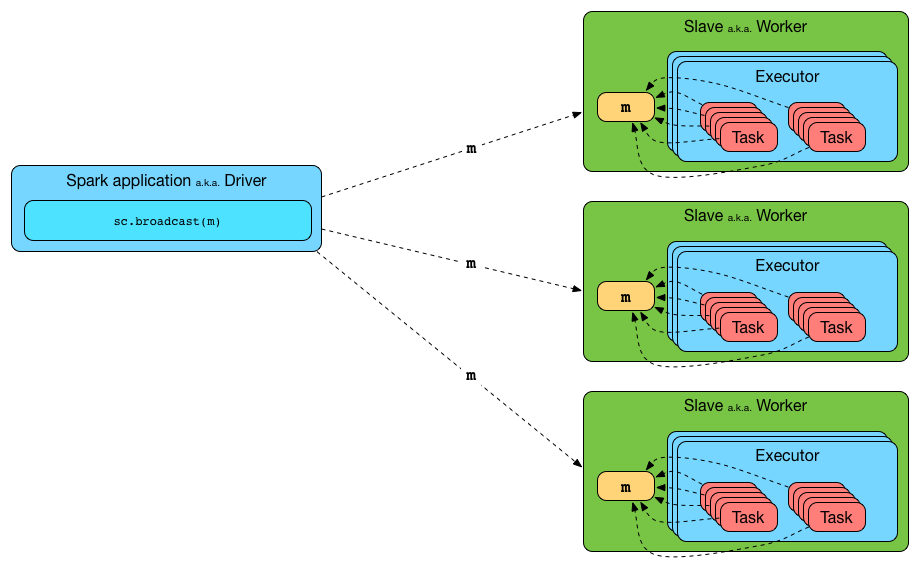
\includegraphics{./_images/sparkcontext-broadcast-executors.png}

(출처:
https://jaceklaskowski.gitbooks.io/mastering-apache-spark/content/spark-broadcast.html)

    Example:

\begin{quote}
유입되는 로그(file\_new\_log)에서 특정 단어들(bv\_lookup\_words)이
포함된 문장만을 처리한다고 해 보자.
\end{quote}

    \begin{Verbatim}[commandchars=\\\{\}]
{\color{incolor}In [{\color{incolor}125}]:} \PY{k}{val} \PY{n}{bv\PYZus{}lookup\PYZus{}words} \PY{k}{=} \PY{n}{sc}\PY{o}{.}\PY{n}{broadcast}\PY{o}{(}\PY{n+nc}{Set}\PY{o}{(}\PY{l+s}{\PYZdq{}spark\PYZdq{}}\PY{o}{,} \PY{l+s}{\PYZdq{}you\PYZdq{}}\PY{o}{,} \PY{l+s}{\PYZdq{}mllib\PYZdq{}}\PY{o}{,} \PY{l+s}{\PYZdq{}python\PYZdq{}}\PY{o}{)}\PY{o}{)}
\end{Verbatim}

    \begin{Verbatim}[commandchars=\\\{\}]
{\color{incolor}In [{\color{incolor}126}]:} \PY{k}{val} \PY{n}{file\PYZus{}new\PYZus{}log} \PY{k}{=} \PY{n}{sc}\PY{o}{.}\PY{n}{textFile}\PY{o}{(}\PY{l+s}{\PYZdq{}/home/sparkuser/spark\PYZhy{}1.6.2\PYZhy{}bin\PYZhy{}hadoop2.6/README.md\PYZdq{}}\PY{o}{)}\PY{o}{.}\PY{n}{repartition}\PY{o}{(}\PY{l+m+mi}{11}\PY{o}{)}
          
          \PY{n}{file\PYZus{}new\PYZus{}log}\PY{o}{.}
            \PY{n}{take}\PY{o}{(}\PY{l+m+mi}{10}\PY{o}{)}\PY{o}{.}
            \PY{n}{foreach}\PY{o}{(}\PY{n}{println}\PY{o}{)}
\end{Verbatim}

    \begin{Verbatim}[commandchars=\\\{\}]

Spark is built using [Apache Maven](http://maven.apache.org/).
The easiest way to start using Spark is through the Scala shell:




["Specifying the Hadoop Version"](http://spark.apache.org/docs/latest/building-spark.html\#specifying-the-hadoop-version)
\# Apache Spark


    \end{Verbatim}

    \begin{Verbatim}[commandchars=\\\{\}]
{\color{incolor}In [{\color{incolor}127}]:} \PY{n}{file\PYZus{}new\PYZus{}log}\PY{o}{.}
            \PY{n}{map}\PY{o}{\PYZob{}} \PY{n}{line} \PY{k}{=\PYZgt{}} 
              \PY{k}{val} \PY{n}{words} \PY{k}{=} \PY{n}{line}\PY{o}{.}\PY{n}{toLowerCase}\PY{o}{(}\PY{o}{)}\PY{o}{.}\PY{n}{split}\PY{o}{(}\PY{l+s}{\PYZdq{} \PYZdq{}}\PY{o}{)}\PY{o}{.}\PY{n}{toSet}\PY{o}{;}
              \PY{k}{val} \PY{n}{common} \PY{k}{=} \PY{n}{words} \PY{o}{\PYZam{}} \PY{n}{bv\PYZus{}lookup\PYZus{}words}\PY{o}{.}\PY{n}{value}\PY{o}{;}
              \PY{k}{if}\PY{o}{(}\PY{n}{common}\PY{o}{.}\PY{n}{size} \PY{o}{\PYZgt{}} \PY{l+m+mi}{0}\PY{o}{)} \PY{o}{(}\PY{n}{common}\PY{o}{,} \PY{n}{line}\PY{o}{)}
              \PY{k}{else} \PY{o}{(}\PY{n+nc}{Set}\PY{o}{(}\PY{o}{)}\PY{o}{,} \PY{n}{line}\PY{o}{)}
            \PY{o}{\PYZcb{}}\PY{o}{.}
            \PY{n}{filter}\PY{o}{\PYZob{}}\PY{k}{case} \PY{o}{(}\PY{n}{k}\PY{o}{,} \PY{n}{v}\PY{o}{)} \PY{k}{=\PYZgt{}} \PY{n}{k}\PY{o}{.}\PY{n}{size} \PY{o}{\PYZgt{}} \PY{l+m+mi}{0}\PY{o}{\PYZcb{}}\PY{o}{.}
            \PY{n}{take}\PY{o}{(}\PY{l+m+mi}{100}\PY{o}{)}\PY{o}{.}
            \PY{n}{foreach}\PY{o}{(}\PY{n}{println}\PY{o}{)}
\end{Verbatim}

    \begin{Verbatim}[commandchars=\\\{\}]
(Set(spark),Spark is built using [Apache Maven](http://maven.apache.org/).)
(Set(spark),The easiest way to start using Spark is through the Scala shell:)
(Set(spark),\# Apache Spark)
(Set(spark),To build Spark and its example programs, run:)
(Set(spark),Spark is a fast and general cluster computing system for Big Data. It provides)
(Set(you, spark),You can find the latest Spark documentation, including a programming)
(Set(you),(You do not need to do this if you downloaded a pre-built package.))
(Set(you),You can set the MASTER environment variable when running examples to submit)
(Set(spark),rich set of higher-level tools including Spark SQL for SQL and DataFrames,)
(Set(spark),Spark uses the Hadoop core library to talk to HDFS and other Hadoop-supported)
(Set(mllib),MLlib for machine learning, GraphX for graph processing,)
(Set(spark),Testing first requires [building Spark](\#building-spark). Once Spark is built, tests)
(Set(spark),and Spark Streaming for stream processing.)
(Set(python),\#\# Interactive Python Shell)
(Set(you),locally with one thread, or "local[N]" to run locally with N threads. You)
(Set(you, spark),Hadoop, you must build Spark against the same version that your cluster runs.)
(Set(spark),\#\# Building Spark)
(Set(spark),Spark also comes with several sample programs in the `examples` directory.)
(Set(you, python),Alternatively, if you prefer Python, you can use the Python shell:)

    \end{Verbatim}

    \begin{quote}
위의 작업을 join transformation을 이용하여 수행할 수도 있지만,\\분산
환경에서는 상대적으로 큰 테이블(fact table)과 작은 테이블(dimension)을
join하는 경우\\map을 이용한 join을 사용하는 것이 효과적(map-size
join이라 함)\\(참고:
http://dmtolpeko.com/2015/02/20/map-side-join-in-spark/)
\end{quote}

    \subsubsection{브로드캐스트 최적화(Optimizing
Broadcasts)}\label{uxbe0cuxb85cuxb4dcuxce90uxc2a4uxd2b8-uxcd5cuxc801uxd654optimizing-broadcasts}

    \begin{quote}
앞서 broadcast variable을 이용한 구현을\\일반 변수를 사용하여 아래와
같이 바꿔볼 수 있다.
\end{quote}

    \begin{Verbatim}[commandchars=\\\{\}]
{\color{incolor}In [{\color{incolor}128}]:} \PY{k}{val} \PY{n}{lookup\PYZus{}words} \PY{k}{=} \PY{n+nc}{Set}\PY{o}{(}\PY{l+s}{\PYZdq{}spark\PYZdq{}}\PY{o}{,} \PY{l+s}{\PYZdq{}you\PYZdq{}}\PY{o}{,} \PY{l+s}{\PYZdq{}mllib\PYZdq{}}\PY{o}{,} \PY{l+s}{\PYZdq{}python\PYZdq{}}\PY{o}{)}
\end{Verbatim}

    \begin{Verbatim}[commandchars=\\\{\}]
{\color{incolor}In [{\color{incolor}129}]:} \PY{k}{val} \PY{n}{file\PYZus{}new\PYZus{}log} \PY{k}{=} \PY{n}{sc}\PY{o}{.}\PY{n}{textFile}\PY{o}{(}\PY{l+s}{\PYZdq{}/home/sparkuser/spark\PYZhy{}1.6.2\PYZhy{}bin\PYZhy{}hadoop2.6/README.md\PYZdq{}}\PY{o}{)}\PY{o}{.}\PY{n}{repartition}\PY{o}{(}\PY{l+m+mi}{11}\PY{o}{)}
          
          \PY{n}{file\PYZus{}new\PYZus{}log}\PY{o}{.}
            \PY{n}{take}\PY{o}{(}\PY{l+m+mi}{10}\PY{o}{)}\PY{o}{.}
            \PY{n}{foreach}\PY{o}{(}\PY{n}{println}\PY{o}{)}
\end{Verbatim}

    \begin{Verbatim}[commandchars=\\\{\}]

Spark is built using [Apache Maven](http://maven.apache.org/).
The easiest way to start using Spark is through the Scala shell:




["Specifying the Hadoop Version"](http://spark.apache.org/docs/latest/building-spark.html\#specifying-the-hadoop-version)
\# Apache Spark


    \end{Verbatim}

    \begin{Verbatim}[commandchars=\\\{\}]
{\color{incolor}In [{\color{incolor}130}]:} \PY{n}{file\PYZus{}new\PYZus{}log}\PY{o}{.}
            \PY{n}{map}\PY{o}{\PYZob{}} \PY{n}{line} \PY{k}{=\PYZgt{}} 
              \PY{k}{val} \PY{n}{words} \PY{k}{=} \PY{n}{line}\PY{o}{.}\PY{n}{toLowerCase}\PY{o}{(}\PY{o}{)}\PY{o}{.}\PY{n}{split}\PY{o}{(}\PY{l+s}{\PYZdq{} \PYZdq{}}\PY{o}{)}\PY{o}{.}\PY{n}{toSet}\PY{o}{;}
              \PY{k}{val} \PY{n}{common} \PY{k}{=} \PY{n}{words} \PY{o}{\PYZam{}} \PY{n}{lookup\PYZus{}words}\PY{o}{;}
              \PY{k}{if}\PY{o}{(}\PY{n}{common}\PY{o}{.}\PY{n}{size} \PY{o}{\PYZgt{}} \PY{l+m+mi}{0}\PY{o}{)} \PY{o}{(}\PY{n}{common}\PY{o}{,} \PY{n}{line}\PY{o}{)}
              \PY{k}{else} \PY{o}{(}\PY{n+nc}{Set}\PY{o}{(}\PY{o}{)}\PY{o}{,} \PY{n}{line}\PY{o}{)}
            \PY{o}{\PYZcb{}}\PY{o}{.}
            \PY{n}{filter}\PY{o}{\PYZob{}}\PY{k}{case} \PY{o}{(}\PY{n}{k}\PY{o}{,} \PY{n}{v}\PY{o}{)} \PY{k}{=\PYZgt{}} \PY{n}{k}\PY{o}{.}\PY{n}{size} \PY{o}{\PYZgt{}} \PY{l+m+mi}{0}\PY{o}{\PYZcb{}}\PY{o}{.}
            \PY{n}{take}\PY{o}{(}\PY{l+m+mi}{100}\PY{o}{)}\PY{o}{.}
            \PY{n}{foreach}\PY{o}{(}\PY{n}{println}\PY{o}{)}
\end{Verbatim}

    \begin{Verbatim}[commandchars=\\\{\}]
(Set(spark),Spark is built using [Apache Maven](http://maven.apache.org/).)
(Set(spark),The easiest way to start using Spark is through the Scala shell:)
(Set(spark),\# Apache Spark)
(Set(spark),To build Spark and its example programs, run:)
(Set(spark),Spark is a fast and general cluster computing system for Big Data. It provides)
(Set(you, spark),You can find the latest Spark documentation, including a programming)
(Set(you),(You do not need to do this if you downloaded a pre-built package.))
(Set(you),You can set the MASTER environment variable when running examples to submit)
(Set(spark),rich set of higher-level tools including Spark SQL for SQL and DataFrames,)
(Set(spark),Spark uses the Hadoop core library to talk to HDFS and other Hadoop-supported)
(Set(mllib),MLlib for machine learning, GraphX for graph processing,)
(Set(spark),Testing first requires [building Spark](\#building-spark). Once Spark is built, tests)
(Set(spark),and Spark Streaming for stream processing.)
(Set(python),\#\# Interactive Python Shell)
(Set(you),locally with one thread, or "local[N]" to run locally with N threads. You)
(Set(you, spark),Hadoop, you must build Spark against the same version that your cluster runs.)
(Set(spark),\#\# Building Spark)
(Set(spark),Spark also comes with several sample programs in the `examples` directory.)
(Set(you, python),Alternatively, if you prefer Python, you can use the Python shell:)

    \end{Verbatim}

    \begin{quote}
위와 같은 구현에서는 lookup\_words의 복사본이 모든 task에
직렬화되어(serialized) 전달되고, 각 task를 실행하기 직전에
역직렬화(deserialized)된다.
\end{quote}

\begin{quote}
물론 broadcast variable을 사용할 경우에도 비슷한 과정을 거치지만 worker
단위로 한번만 직렬화 개체를 전달하고 역직렬화(deserialized)가 한번만
필요하므로 반복사용되는 데이터의 경우 효과적이다.
\end{quote}

\begin{quote}
따라서 network overhead를 줄일 수 있고 직렬화(serialization) 포멧을
사용하는 것이 매우 중요하다.
\end{quote}

\begin{quote}
8장에서 $Kyro$라는 빠른 직렬화 라이브러리에 대해 배우게 될 것이다.
\end{quote}

    \subsubsection{파티션별로 작업하기(Working on a Per-Partition
Basis)}\label{uxd30cuxd2f0uxc158uxbcc4uxb85c-uxc791uxc5c5uxd558uxae30working-on-a-per-partition-basis}

    \begin{quote}
RDD의 각 element에 대하여 어떤 작업을 하는 것이 아니라\\각 Partition에
대하여 한번식 어떤 작업이 해야하는 경우\\예를들어 DB connection이나
난수생성등의 일은 data element단위로 필요한 일이 아니라\\partition단위로
필요한 작업니다.
\end{quote}

\begin{quote}
이런 partition단위의 일을 쉽게 해 주는 것이 \textbf{mapPartitions,
mapPartitionsWithIndex, foreachPartition}함수이다.
\end{quote}

    \begin{Verbatim}[commandchars=\\\{\}]
{\color{incolor}In [{\color{incolor}150}]:} \PY{k}{import} \PY{n+nn}{scala.collection.mutable.HashMap}
          \PY{k}{import} \PY{n+nn}{org.apache.spark.TaskContext}
          
          \PY{k}{val} \PY{n}{file\PYZus{}new\PYZus{}log} \PY{k}{=} \PY{n}{sc}\PY{o}{.}\PY{n}{textFile}\PY{o}{(}\PY{l+s}{\PYZdq{}/home/sparkuser/spark\PYZhy{}1.6.2\PYZhy{}bin\PYZhy{}hadoop2.6/README.md\PYZdq{}}\PY{o}{)}\PY{o}{.}\PY{n}{repartition}\PY{o}{(}\PY{l+m+mi}{30}\PY{o}{)}
          
          \PY{n}{file\PYZus{}new\PYZus{}log}\PY{o}{.}
            \PY{n}{mapPartitions}\PY{o}{(}\PY{n}{lineIter} \PY{k}{=\PYZgt{}} \PY{o}{\PYZob{}}
                
                \PY{k}{val} \PY{n}{work2do} \PY{k}{=} \PY{l+s}{\PYZdq{}Common work for partition \PYZdq{}} \PY{o}{+} \PY{n+nc}{TaskContext}\PY{o}{.}\PY{n}{get}\PY{o}{.}\PY{n}{partitionId}
                
                \PY{n}{lineIter}\PY{o}{.}\PY{n}{toList}\PY{o}{.}\PY{n}{map}\PY{o}{(}\PY{n}{line} \PY{k}{=\PYZgt{}} \PY{n}{work2do} \PY{o}{+} \PY{l+s}{\PYZdq{} \PYZhy{}\PYZgt{} \PYZdq{}} \PY{o}{+} \PY{n}{line}\PY{o}{)}\PY{o}{.}\PY{n}{iterator}
              \PY{o}{\PYZcb{}}
            \PY{o}{)}\PY{o}{.}
            \PY{n}{take}\PY{o}{(}\PY{l+m+mi}{15}\PY{o}{)}\PY{o}{.}
            \PY{n}{foreach}\PY{o}{(}\PY{n}{println}\PY{o}{)}
\end{Verbatim}

    \begin{Verbatim}[commandchars=\\\{\}]
Common work for partition 0 -> 
Common work for partition 0 -> You can set the MASTER environment variable when running examples to submit
Common work for partition 0 -> building for particular Hive and Hive Thriftserver distributions.
Common work for partition 1 -> \# Apache Spark
Common work for partition 1 -> \#\# Interactive Scala Shell
Common work for partition 1 -> examples to a cluster. This can be a mesos:// or spark:// URL,
Common work for partition 1 -> 
Common work for partition 2 -> 
Common work for partition 2 -> 
Common work for partition 2 -> "yarn" to run on YARN, and "local" to run
Common work for partition 2 -> \#\# Configuration
Common work for partition 3 -> Spark is a fast and general cluster computing system for Big Data. It provides
Common work for partition 3 -> The easiest way to start using Spark is through the Scala shell:
Common work for partition 3 -> locally with one thread, or "local[N]" to run locally with N threads. You
Common work for partition 3 -> 

    \end{Verbatim}

    \begin{Verbatim}[commandchars=\\\{\}]
{\color{incolor}In [{\color{incolor}151}]:} \PY{k}{import} \PY{n+nn}{scala.collection.mutable.HashMap}
          \PY{k}{import} \PY{n+nn}{org.apache.spark.TaskContext}
          
          \PY{k}{val} \PY{n}{file\PYZus{}new\PYZus{}log} \PY{k}{=} \PY{n}{sc}\PY{o}{.}\PY{n}{textFile}\PY{o}{(}\PY{l+s}{\PYZdq{}/home/sparkuser/spark\PYZhy{}1.6.2\PYZhy{}bin\PYZhy{}hadoop2.6/README.md\PYZdq{}}\PY{o}{)}\PY{o}{.}\PY{n}{repartition}\PY{o}{(}\PY{l+m+mi}{30}\PY{o}{)}
          
          \PY{n}{file\PYZus{}new\PYZus{}log}\PY{o}{.}
            \PY{n}{mapPartitionsWithIndex}\PY{o}{(}\PY{o}{(}\PY{n}{idx}\PY{o}{,} \PY{n}{lineIter}\PY{o}{)} \PY{k}{=\PYZgt{}} \PY{o}{\PYZob{}}
                
                \PY{k}{val} \PY{n}{work2do} \PY{k}{=} \PY{l+s}{\PYZdq{}Common work for partition \PYZdq{}} \PY{o}{+} \PY{n}{idx}
                
                \PY{n}{lineIter}\PY{o}{.}\PY{n}{toList}\PY{o}{.}\PY{n}{map}\PY{o}{(}\PY{n}{line} \PY{k}{=\PYZgt{}} \PY{n}{work2do} \PY{o}{+} \PY{l+s}{\PYZdq{} \PYZhy{}\PYZgt{} \PYZdq{}} \PY{o}{+} \PY{n}{line}\PY{o}{)}\PY{o}{.}\PY{n}{iterator}
              \PY{o}{\PYZcb{}}
            \PY{o}{)}\PY{o}{.}
            \PY{n}{take}\PY{o}{(}\PY{l+m+mi}{15}\PY{o}{)}\PY{o}{.}
            \PY{n}{foreach}\PY{o}{(}\PY{n}{println}\PY{o}{)}
\end{Verbatim}

    \begin{Verbatim}[commandchars=\\\{\}]
Common work for partition 0 -> 
Common work for partition 0 -> You can set the MASTER environment variable when running examples to submit
Common work for partition 0 -> building for particular Hive and Hive Thriftserver distributions.
Common work for partition 1 -> \# Apache Spark
Common work for partition 1 -> \#\# Interactive Scala Shell
Common work for partition 1 -> examples to a cluster. This can be a mesos:// or spark:// URL,
Common work for partition 1 -> 
Common work for partition 2 -> 
Common work for partition 2 -> 
Common work for partition 2 -> "yarn" to run on YARN, and "local" to run
Common work for partition 2 -> \#\# Configuration
Common work for partition 3 -> Spark is a fast and general cluster computing system for Big Data. It provides
Common work for partition 3 -> The easiest way to start using Spark is through the Scala shell:
Common work for partition 3 -> locally with one thread, or "local[N]" to run locally with N threads. You
Common work for partition 3 -> 

    \end{Verbatim}

    \subsubsection{외부 프로그램과 파이프로 연결하기(Piping to External
Programs)}\label{uxc678uxbd80-uxd504uxb85cuxadf8uxb7a8uxacfc-uxd30cuxc774uxd504uxb85c-uxc5f0uxacb0uxd558uxae30piping-to-external-programs}

    \begin{quote}
\textbf{pipe} 함수를 이용하여\\RDD의 데이터를 (Scala, Java, Python이
아니더라도) 스크립트에 전달하고\\처리된 결과값을 받아올 수 있다.
\end{quote}

\begin{quote}
SparkContext.addFile(path) 와 같이 context에 file을 추가하면,\\driver
node에 존재하는 script file이 각 worker node에 복제된다.
\end{quote}

\begin{quote}
각 node에서 file의 위치는 SparkFiles.getRootDirectory를 이용하여 알수
있다.
\end{quote}

\begin{quote}
또한 SparkFiles.get(name)으로 각 node에서 file을 복제해갈 수 있다.\\물론
수동 혹은 다른 방법으로 각 worker node의 SparkFiles.getRootDirectory
경로에 위치시켜도 된다.
\end{quote}

    \begin{quote}
예제로 문장을 받아 " ``으로 나눈 후 단어 수를 반환하는 아래의 R script를
테스트
\end{quote}

    \begin{Shaded}
\begin{Highlighting}[]
\CommentTok{#!/usr/bin/Rscript}
\NormalTok{f <-}\StringTok{ }\KeywordTok{file}\NormalTok{(}\StringTok{"stdin"}\NormalTok{)}
\KeywordTok{open}\NormalTok{(f)}

\NormalTok{while(}\KeywordTok{length}\NormalTok{(line <-}\StringTok{ }\KeywordTok{readLines}\NormalTok{(f, }\DataTypeTok{n=}\DecValTok{1}\NormalTok{)) >}\StringTok{ }\DecValTok{0}\NormalTok{) \{}
  \NormalTok{len <-}\StringTok{ }\KeywordTok{length}\NormalTok{(}\KeywordTok{strsplit}\NormalTok{(line, }\StringTok{" "}\NormalTok{)[[}\DecValTok{1}\NormalTok{]])}
  \KeywordTok{write}\NormalTok{(len, }\KeywordTok{stdout}\NormalTok{())}
\NormalTok{\}}
\end{Highlighting}
\end{Shaded}

    \begin{Verbatim}[commandchars=\\\{\}]
{\color{incolor}In [{\color{incolor}1}]:} \PY{k}{val} \PY{n}{file\PYZus{}new\PYZus{}log} \PY{k}{=} \PY{n}{sc}\PY{o}{.}\PY{n}{textFile}\PY{o}{(}\PY{l+s}{\PYZdq{}/home/sparkuser/spark\PYZhy{}1.6.2\PYZhy{}bin\PYZhy{}hadoop2.6/README.md\PYZdq{}}\PY{o}{)}\PY{o}{.}\PY{n}{repartition}\PY{o}{(}\PY{l+m+mi}{11}\PY{o}{)}
        
        \PY{n}{file\PYZus{}new\PYZus{}log}\PY{o}{.}
          \PY{n}{filter}\PY{o}{(}\PY{n}{line} \PY{k}{=\PYZgt{}} \PY{n}{line} \PY{o}{!=} \PY{l+s}{\PYZdq{}\PYZdq{}}\PY{o}{)}\PY{o}{.}
          \PY{n}{take}\PY{o}{(}\PY{l+m+mi}{10}\PY{o}{)}\PY{o}{.}
          \PY{n}{foreach}\PY{o}{(}\PY{n}{println}\PY{o}{)}
\end{Verbatim}

    \begin{Verbatim}[commandchars=\\\{\}]
Spark is built using [Apache Maven](http://maven.apache.org/).
The easiest way to start using Spark is through the Scala shell:
["Specifying the Hadoop Version"](http://spark.apache.org/docs/latest/building-spark.html\#specifying-the-hadoop-version)
\# Apache Spark
To build Spark and its example programs, run:
    ./bin/pyspark
    ./bin/run-example SparkPi
    MASTER=spark://host:7077 ./bin/run-example SparkPi
Please see the guidance on how to
for detailed guidance on building for a particular distribution of Hadoop, including

    \end{Verbatim}

    \begin{Verbatim}[commandchars=\\\{\}]
{\color{incolor}In [{\color{incolor}2}]:} \PY{k}{import} \PY{n+nn}{org.apache.spark.SparkFiles}
        
        \PY{k}{val} \PY{n}{rScript} \PY{k}{=} \PY{l+s}{\PYZdq{}/home/sparkuser/work/jupyter/\PYZus{}etc/withSpark.R\PYZdq{}}
        \PY{k}{val} \PY{n}{rScriptName} \PY{k}{=} \PY{l+s}{\PYZdq{}withSpark.R\PYZdq{}}
        \PY{n}{sc}\PY{o}{.}\PY{n}{addFile}\PY{o}{(}\PY{n}{rScript}\PY{o}{)}
\end{Verbatim}

    \begin{Verbatim}[commandchars=\\\{\}]
{\color{incolor}In [{\color{incolor}3}]:} \PY{n}{file\PYZus{}new\PYZus{}log}\PY{o}{.}
          \PY{n}{filter}\PY{o}{(}\PY{n}{line} \PY{k}{=\PYZgt{}} \PY{n}{line} \PY{o}{!=} \PY{l+s}{\PYZdq{}\PYZdq{}}\PY{o}{)}\PY{o}{.}
          \PY{n}{pipe}\PY{o}{(}\PY{n+nc}{Seq}\PY{o}{(}\PY{n+nc}{SparkFiles}\PY{o}{.}\PY{n}{get}\PY{o}{(}\PY{n}{rScriptName}\PY{o}{)}\PY{o}{)}\PY{o}{)}\PY{o}{.}
          \PY{n}{collect}\PY{o}{(}\PY{o}{)}\PY{o}{.}\PY{n}{toList}
\end{Verbatim}

            \begin{Verbatim}[commandchars=\\\{\}]
{\color{outcolor}Out[{\color{outcolor}3}]:} List(6, 12, 4, 3, 8, 5, 6, 7, 7, 12, 3, 5, 8, 8, 14, 8, 10, 6, 13, 13, 10, 8, 6, 2, 11, 6, 13, 6, 12, 3, 12, 3, 10, 8, 12, 13, 6, 8, 8, 2, 3, 9, 10, 11, 12, 6, 4, 13, 4, 13, 3, 4, 11, 14, 1, 11, 11, 3, 5, 7)
\end{Verbatim}
        
    \subsubsection{수치 RDD 연산들(Numeric RDD
Operations)}\label{uxc218uxce58-rdd-uxc5f0uxc0b0uxb4e4numeric-rdd-operations}

    \begin{quote}
수치 데이터를 포함하는 RDD의 기술통계량(descriptive statistics)을
계산하기 위한 함수들을 제공한다.\\count(), mean(), sum(), max(), min(),
variance(), sampleVariance(), stdev(), sampleStddev()
\end{quote}

    \begin{quote}
예제로 문장내 단어의 수가\\파일내 문장들의 단어수 분포의\\평균을
중심으로 68\% 내에 있는 문장들을 필터링 해 보자.
\end{quote}

    \begin{figure}[htbp]
\centering
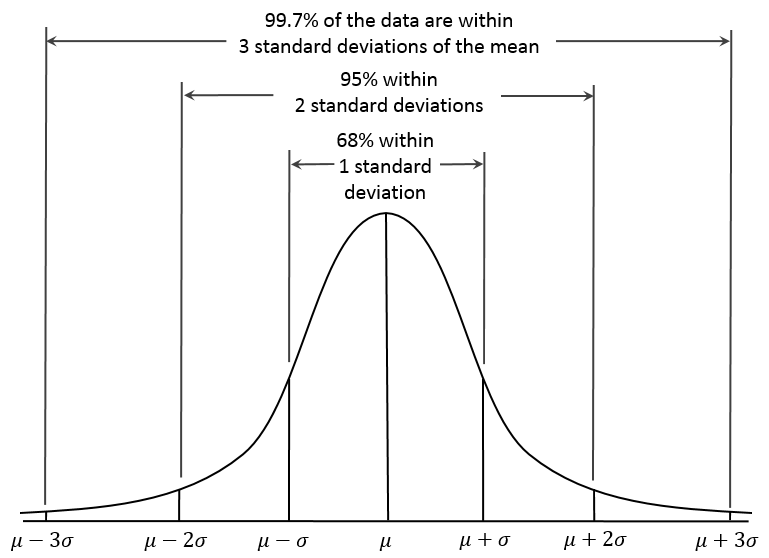
\includegraphics{./_images/Empirical_Rule.PNG}
\caption{Local image}
\end{figure}

    \begin{Verbatim}[commandchars=\\\{\}]
{\color{incolor}In [{\color{incolor}25}]:} \PY{k}{val} \PY{n}{file\PYZus{}new\PYZus{}log} \PY{k}{=} \PY{n}{sc}\PY{o}{.}\PY{n}{textFile}\PY{o}{(}\PY{l+s}{\PYZdq{}/home/sparkuser/spark\PYZhy{}1.6.2\PYZhy{}bin\PYZhy{}hadoop2.6/README.md\PYZdq{}}\PY{o}{)}\PY{o}{.}\PY{n}{repartition}\PY{o}{(}\PY{l+m+mi}{11}\PY{o}{)}
         
         \PY{n}{file\PYZus{}new\PYZus{}log}\PY{o}{.}
           \PY{n}{filter}\PY{o}{(}\PY{n}{line} \PY{k}{=\PYZgt{}} \PY{n}{line} \PY{o}{!=} \PY{l+s}{\PYZdq{}\PYZdq{}}\PY{o}{)}\PY{o}{.}
           \PY{n}{map}\PY{o}{(}\PY{n}{line} \PY{k}{=\PYZgt{}} \PY{o}{(}\PY{n}{line}\PY{o}{.}\PY{n}{split}\PY{o}{(}\PY{l+s}{\PYZdq{} \PYZdq{}}\PY{o}{)}\PY{o}{.}\PY{n}{length}\PY{o}{,} \PY{n}{line}\PY{o}{)}\PY{o}{)}\PY{o}{.}
           \PY{n}{take}\PY{o}{(}\PY{l+m+mi}{10}\PY{o}{)}\PY{o}{.}
           \PY{n}{foreach}\PY{o}{(}\PY{n}{println}\PY{o}{)}
\end{Verbatim}

    \begin{Verbatim}[commandchars=\\\{\}]
(6,Spark is built using [Apache Maven](http://maven.apache.org/).)
(12,The easiest way to start using Spark is through the Scala shell:)
(4,["Specifying the Hadoop Version"](http://spark.apache.org/docs/latest/building-spark.html\#specifying-the-hadoop-version))
(3,\# Apache Spark)
(8,To build Spark and its example programs, run:)
(5,    ./bin/pyspark)
(6,    ./bin/run-example SparkPi)
(7,    MASTER=spark://host:7077 ./bin/run-example SparkPi)
(7,Please see the guidance on how to)
(12,for detailed guidance on building for a particular distribution of Hadoop, including)

    \end{Verbatim}

    \begin{Verbatim}[commandchars=\\\{\}]
{\color{incolor}In [{\color{incolor}26}]:} \PY{k}{val} \PY{n}{lineLen} \PY{k}{=} \PY{n}{file\PYZus{}new\PYZus{}log}\PY{o}{.}
           \PY{n}{filter}\PY{o}{(}\PY{n}{line} \PY{k}{=\PYZgt{}} \PY{n}{line} \PY{o}{!=} \PY{l+s}{\PYZdq{}\PYZdq{}}\PY{o}{)}\PY{o}{.}
           \PY{n}{map}\PY{o}{(}\PY{n}{line} \PY{k}{=\PYZgt{}} \PY{n}{line}\PY{o}{.}\PY{n}{split}\PY{o}{(}\PY{l+s}{\PYZdq{} \PYZdq{}}\PY{o}{)}\PY{o}{.}\PY{n}{length}\PY{o}{)}\PY{o}{.}
           \PY{n}{cache}\PY{o}{(}\PY{o}{)}
\end{Verbatim}

    \begin{Verbatim}[commandchars=\\\{\}]
{\color{incolor}In [{\color{incolor}28}]:} \PY{k}{val} \PY{n}{stddev} \PY{k}{=} \PY{n}{lineLen}\PY{o}{.}\PY{n}{stdev}\PY{o}{(}\PY{o}{)}
         \PY{k}{val} \PY{n}{mean} \PY{k}{=} \PY{n}{lineLen}\PY{o}{.}\PY{n}{mean}\PY{o}{(}\PY{o}{)}
         \PY{n}{println}\PY{o}{(}\PY{l+s}{\PYZdq{}stddev: \PYZdq{}} \PY{o}{+} \PY{n}{stddev} \PY{o}{+} \PY{l+s}{\PYZdq{}, mean: \PYZdq{}} \PY{o}{+} \PY{n}{mean}\PY{o}{)}
\end{Verbatim}

    \begin{Verbatim}[commandchars=\\\{\}]
stddev: 3.653613127971938, mean: 7.866666666666665

    \end{Verbatim}

    \begin{Verbatim}[commandchars=\\\{\}]
{\color{incolor}In [{\color{incolor}29}]:} \PY{n}{file\PYZus{}new\PYZus{}log}\PY{o}{.}
           \PY{n}{filter}\PY{o}{(}\PY{n}{line} \PY{k}{=\PYZgt{}} \PY{n}{line} \PY{o}{!=} \PY{l+s}{\PYZdq{}\PYZdq{}}\PY{o}{)}\PY{o}{.}
           \PY{n}{map}\PY{o}{(}\PY{n}{line} \PY{k}{=\PYZgt{}} \PY{o}{(}\PY{n}{line}\PY{o}{.}\PY{n}{split}\PY{o}{(}\PY{l+s}{\PYZdq{} \PYZdq{}}\PY{o}{)}\PY{o}{.}\PY{n}{length}\PY{o}{,} \PY{n}{line}\PY{o}{)}\PY{o}{)}\PY{o}{.}
           \PY{n}{filter}\PY{o}{\PYZob{}}\PY{k}{case} \PY{o}{(}\PY{n}{k}\PY{o}{,} \PY{n}{v}\PY{o}{)} \PY{k}{=\PYZgt{}} \PY{n}{math}\PY{o}{.}\PY{n}{abs}\PY{o}{(}\PY{n}{k} \PY{o}{\PYZhy{}} \PY{n}{mean}\PY{o}{)} \PY{o}{\PYZlt{}} \PY{n}{stddev}\PY{o}{\PYZcb{}}\PY{o}{.}
           \PY{n}{take}\PY{o}{(}\PY{l+m+mi}{10}\PY{o}{)}\PY{o}{.}
           \PY{n}{foreach}\PY{o}{(}\PY{n}{println}\PY{o}{)}
\end{Verbatim}

    \begin{Verbatim}[commandchars=\\\{\}]
(6,Spark is built using [Apache Maven](http://maven.apache.org/).)
(8,To build Spark and its example programs, run:)
(5,    ./bin/pyspark)
(6,    ./bin/run-example SparkPi)
(7,    MASTER=spark://host:7077 ./bin/run-example SparkPi)
(7,Please see the guidance on how to)
(5,    ./bin/spark-shell)
(8,[run tests for a module, or individual tests](https://cwiki.apache.org/confluence/display/SPARK/Useful+Developer+Tools).)
(8,building for particular Hive and Hive Thriftserver distributions.)
(8,    build/mvn -DskipTests clean package)

    \end{Verbatim}

    \begin{Verbatim}[commandchars=\\\{\}]
{\color{incolor}In [{\color{incolor}30}]:} \PY{n}{file\PYZus{}new\PYZus{}log}\PY{o}{.}
           \PY{n}{filter}\PY{o}{(}\PY{n}{line} \PY{k}{=\PYZgt{}} \PY{n}{line} \PY{o}{!=} \PY{l+s}{\PYZdq{}\PYZdq{}}\PY{o}{)}\PY{o}{.}
           \PY{n}{map}\PY{o}{(}\PY{n}{line} \PY{k}{=\PYZgt{}} \PY{o}{(}\PY{n}{line}\PY{o}{.}\PY{n}{split}\PY{o}{(}\PY{l+s}{\PYZdq{} \PYZdq{}}\PY{o}{)}\PY{o}{.}\PY{n}{length}\PY{o}{,} \PY{n}{line}\PY{o}{)}\PY{o}{)}\PY{o}{.}
           \PY{n}{filter}\PY{o}{\PYZob{}}\PY{k}{case} \PY{o}{(}\PY{n}{k}\PY{o}{,} \PY{n}{v}\PY{o}{)} \PY{k}{=\PYZgt{}} \PY{n}{math}\PY{o}{.}\PY{n}{abs}\PY{o}{(}\PY{n}{k} \PY{o}{\PYZhy{}} \PY{n}{mean}\PY{o}{)} \PY{o}{\PYZgt{}} \PY{n}{stddev}\PY{o}{\PYZcb{}}\PY{o}{.}
           \PY{n}{take}\PY{o}{(}\PY{l+m+mi}{10}\PY{o}{)}\PY{o}{.}
           \PY{n}{foreach}\PY{o}{(}\PY{n}{println}\PY{o}{)}
\end{Verbatim}

    \begin{Verbatim}[commandchars=\\\{\}]
(12,The easiest way to start using Spark is through the Scala shell:)
(4,["Specifying the Hadoop Version"](http://spark.apache.org/docs/latest/building-spark.html\#specifying-the-hadoop-version))
(3,\# Apache Spark)
(12,for detailed guidance on building for a particular distribution of Hadoop, including)
(3,\#\# Online Documentation)
(14,Spark is a fast and general cluster computing system for Big Data. It provides)
(13,Many of the example programs print usage help if no params are given.)
(13,high-level APIs in Scala, Java, Python, and R, and an optimized engine that)
(2,\#\# Configuration)
(13,(You do not need to do this if you downloaded a pre-built package.))

    \end{Verbatim}


    % Add a bibliography block to the postdoc
    
    
    
    \end{document}
